%% 使用 jnuthesis 文档类生成南京大学学位论文的示例文档
%%
%% 作者:胡海星,starfish (at) gmail (dot) com
%% 项目主页: http://haixing-hu.github.io/jnu-thesis/
%%
%% 本样例文档中用到了吕琦同学的博士论文的提高和部分内容,在此对他表示感谢.
%%

%% jnuthesis 文档类的可选参数有:
%%   nobackinfo 取消封二页导师签名信息.注意,按照南大的规定,是需要签名页的.
%%   phd/master/bachelor 选择博士/硕士/学士论文

% 使用 blindtext 宏包自动生成章节文字
% 这仅仅是用于生成样例文档,正式论文中一般用不到该宏包
\documentclass[bachelor,winfonts]{jnuthesis}

% 本科课程设计课程名称
\usepackage{graphicx}
\usepackage{subcaption}

\graphicspath{ {images/} }
%%%%%%%%%%%%%%%%%%%%%%%%%%%%%%%%%%%%%%%%%%%%%%%%%%%%%%%%%%%%%%%%%%%%%%%%%%%%%%%
% 设置论文的中文封面

% 如果论文标题过长,可以分两行,第一行用\titlea{}定义,第二行用\titleb{}定义,将上面的\title{}注释掉
\titlea{融合句子结构信息的文本理解}
\titleb{}

% 论文作者姓名
\author{胡勇}
% 论文作者学生证号
\studentnum{1030614418}
% 导师姓名职称
\supervisor{王澜}
\supervisorpos{讲师}
% 第二行导师姓名职称,仿照第一行填写,没有则留空
\supervisorb{}
\supervisorbpos{}
% 论文作者的学科与专业方向
\major{物联网工程}
% 论文作者所在院系的中文名称,学士学位论文此处不带“学院”二字
\department{物联网工程}
% 论文作者所在学校或机构的名称.此属性可选,默认值为``江南大学''.
\institute{江南大学}
% 学士学位获得日期,需设置年、月,默认为编译日期.
\bachelordegreeyear{2018}
\bachelordegreemonth{6}
%%%%%%%%%%%%%%%%%%%%%%%%%%%%%%%%%%%%%%%%%%%%%%%%%%%%%%%%%%%%%%%%%%%%%%%%%%%%%%%

%-------------------------------------------------------------------------------
%	CODE INCLUSION CONFIGURATION
%-------------------------------------------------------------------------------
\usepackage{listings}
\newfontfamily\menlo{Menlo}
\usepackage{color}
\lstset{
    columns=fixed,
    breaklines=true,
    numbers=left,                                        % 在左侧显示行号
    frame=single,                                        % 显示背景边框
    % backgroundcolor=\color[RGB]{245,245,244},            % 设定背景颜色
    % keywordstyle=\color[RGB]{40,40,255},                 % 设定关键字颜色
    numberstyle=\footnotesize\color{darkgray},           % 设定行号格式
    % commentstyle=\color[RGB]{0,96,96},                   % 设置代码注释的格式
    % stringstyle=\color[RGB]{128,0,0},                    % 设置字符串格式
    showstringspaces=false,                              % 不显示字符串中的空格
    basicstyle=\small\menlo,
    numberstyle=\scriptsize\menlo,
    xleftmargin=0cm,
    xrightmargin=0cm
}

\begin{document}

%%%%%%%%%%%%%%%%%%%%%%%%%%%%%%%%%%%%%%%%%%%%%%%%%%%%%%%%%%%%%%%%%%%%%%%%%%%%%%%

% 制作中文封面
\maketitle

%%%%%%%%%%%%%%%%%%%%%%%%%%%%%%%%%%%%%%%%%%%%%%%%%%%%%%%%%%%%%%%%%%%%%%%%%%%%%%%
% % 开始前言部分
% \frontmatter

%%%%%%%%%%%%%%%%%%%%%%%%%%%%%%%%%%%%%%%%%%%%%%%%%%%%%%%%%%%%%%%%%%%%%%%%%%%%%%%
% 论文的中文摘要
\begin{abstract}
自然语言理解是自然语言处理乃至人工智能领域亟待研究重点与难点,
对其研究在理论上和实际应用上都有重要的意义.
近几年随着深度学习的发展,基于循环神经网络(RNN)、长短期记忆网络(LSTM)等的序列建模方式已经成为了
自然语言处理的主流方法.
但是这些深度学习模型需要大规模训练数据,并且将复杂的语言分析和理解
过程简化成“黒盒子”,难以融合先验语言知识,进而使模型缺乏可解释性.

本文尝试将先验文本语言学知识引入传统深度学习模型中,提出了融合句法结构的深度神经网络.
该模型通过依存句法分析工具获得文本的句法子结构,
然后将文本的语义表示和结构表示分别通过两个独立的LSTM模型,
将子结构输出的加权平均结果与主文本句子的输出结果相融合,
从而实现利用句法结构信息对句子表示增强,最后将这个增强表示送入后续的神经网络中以完成文本分类、机器翻译等文本理解的应用.

通过在文本理解的基础性任务文本分类上进行对照实验,
得出融合模型相对传统深度学习模型具有以下两个主要优点:
(1)由于引入了语言学知识,在小规模数据集上有明显优势;在大规模数据集上也有一定优势,模型有较好的鲁棒性.
(2)通过Attention机制可视化文本中不同结构的重要程度,使得模型具有一定的可解释性.

在实验中还对融合模型的Attention机制和融合方式进行了深入的研究.最终在AGNews数据集上,
融合模型相对于LSTM模型在测试集上的正确率提升了2.5\%.

% 中文关键词.关键词之间用中文全角分号隔开,末尾无标点符号.
\keywords{文本理解;依存句法结构;深度学习;融合模型}
\end{abstract}

%%%%%%%%%%%%%%%%%%%%%%%%%%%%%%%%%%%%%%%%%%%%%%%%%%%%%%%%%%%%%%%%%%%%%%%%%%%%%%%
% 论文的英文摘要



\begin{englishabstract}
Natural language understanding is an urgent research focus and difficulty in the field of natural language processing and artificial intelligence.
The research is of great significance in both theory and practice.
In recent years, with the development of deep learning, the sequential modeling methods based on Recurrent Neural Network (RNN) and Long Short Term Memory Network (LSTM) have been established.
and these model has been the  mainstream way of natural language processing.
But these deep learning models require massive training data, and the model is all in the black box of the neural network.
The whole model lacks the interpretability and robustness.
Moreover, the model ignores the syntactic structure and other linguistic knowledge in the text, which can be used to improve the model.

This paper attempts to introduce the knowledge of prior text linguistics into the traditional deep learning model, and puts forward the deep neural network of syntactic structure.
This model acquires the syntactic substructure of text by means of the dependency syntactic analysis tool.
Then the main text sentence and syntactic substructure are respectively adopted by two independent LSTM models.
The weighted average result of the substructure output is combined with the output result of the main text sentence.
A final fusion representation is obtained, which is then sent to the subsequent neural network to complete the application of text classification, machine translation and other text understanding.

By conducting a controlled experiment on the basic task text categorization of text comprehension,
It is concluded that the fusion model has the following advantages compared with the traditional deep learning model:
(1) due to the introduction of linguistic knowledge, there are obvious advantages in the small-scale data set; There are some advantages in large-scale data sets, and the model has good robustness.
(2) the importance of different structures in the visual text of the Attention mechanism makes the model have certain interpretability.

In the experiment, the Attention mechanism and fusion mode of the fusion model were further studied. Finally, in the AGNews data set,
The accuracy of the fusion model in the test set was increased by 2.5\% compared with the LSTM model.
% 英文关键词.关键词之间用英文半角逗号隔开,末尾无符号.
\englishkeywords{Text understanding;Structure of dependency syntax; Deep learning; Fusion model}
\end{englishabstract}

%%%%%%%%%%%%%%%%%%%%%%%%%%%%%%%%%%%%%%%%%%%%%%%%%%%%%%%%%%%%%%%%%%%%%%%%%%%%%%%
% 生成论文目次
\tableofcontents

%%%%%%%%%%%%%%%%%%%%%%%%%%%%%%%%%%%%%%%%%%%%%%%%%%%%%%%%%%%%%%%%%%%%%%%%%%%%%%%
% 开始正文部分
\mainmatter

%%%%%%%%%%%%%%%%%%%%%%%%%%%%%%%%%%%%%%%%%%%%%%%%%%%%%%%%%%%%%%%%%%%%%%%%%%%%%%%
% 学位论文的正文应以《绪论》作为第一章

%第一章绪论
\chapter{绪论}\label{chapter_introduction}
\section{研究背景和意义}
自然语言处理(Natural Language Processing,NLP)是研究计算机处理人类语言的一门技术,也是人工智能(Artificial Intelligence,AI)最初发展的切入点和当前关注的焦点.

人工智能体系可分为运算智能、感知智能、认知智能三个层次(图1-1).其中,最后的认知智能的发展主要体现为自然语言处理技术的进步.
如果语言智能够实现突破,与它同属认知智能的知识和推理就会得到长足的发展,进而推动整个人工智能体系进步,让更多的应用场景落地.
所以自然语言处理技术也被认为是人工智能皇冠上的明珠.

而自然语言理解(Natural Language Understanding,NLU)技术则是对语义信息的深层次挖掘和处理,是NLP技术当前研究的重点和难点.
广义的自然语言理解可以分为两类,第一类是针对口语内容的理解,如语音识别,语音解析和语音合成;
第二类是对书面文本的理解,也是本文主要讨论的内容,即本文题中的文本理解(Text understanding).
人工智能,自然语言处理,自然语言理解和文本理解的关系可以表示为下图.

\begin{figure}[h!]
  \centering
  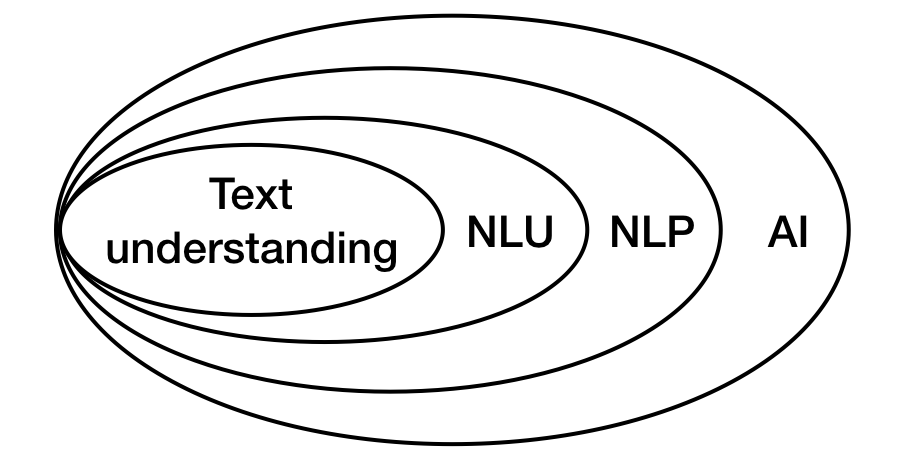
\includegraphics[width=0.5\linewidth]{结构关系.png}
  \caption{人工智能,自然语言处理,自然语言理解和文本理解的关系}
\end{figure}

文本理解技术是众多高级NLP应用不合或缺的一项核心技术,这些应用包括文本分类、信息抽取、自动摘要、机器翻译、问答系统等.

(1)文本分类:文本分类是文本处理中的一个重要模块,它的应用也非常广泛,比如:垃圾过滤、新闻分类、词性标注等.
它和其他的分类没有本质的区别,核心方法为首先提取分类数据的特征,然后选择最优的匹配,从而分类.

(2)信息抽取:信息抽取 是把文本里包含的信息进行结构化处理,变成表格一样的组织形式.
输入信息抽取系统的是原始文本,输出的是固定格式的信息点.
信息点从各种各样的文档中被抽取出来,然后以统一的形式集成在一起.

(3)自动摘要:随着近几年文本信息的爆发式增长,人们每天能接触到海量的文本信息,如新闻、博客、聊天、报告、论文、微博等.
从大量文本信息中提取重要的内容,已成为我们的一个迫切需求,而自动文本摘要就提供了一个高效的解决方案,
可以从原文本中提炼出简洁而重要的信息.

(4)机器翻译:机器翻译,又称为自动翻译,是利用计算机将一种自然语言(源语言)转换为另一种自然语言(目标语言)的过程.
它是计算语言学的一个分支,是人工智能的终极目标之一,具有重要的科学研究价值.
同时,机器翻译又具有重要的实用价值.随着经济全球化及互联网的飞速发展,机器翻译技术在促进政治、经济、文化交流等方面起到越来越重要的作用.

(5)问答系统:问答系统是信息检索系统的一种高级形式,它能用准确、简洁的自然语言回答用户用自然语言提出的问题.
这种交互一直认为是最自然的人机交互方式,随着苹果Siri,微软Cortana,天猫智能客服的推出,智能问答系统成为备受关注的热点研究方向.

(6)舆情分析:舆情是指社会空间中群众对社会事件发生,发展,变化持有的态度、意见、情绪等表现的总和.
网络中的舆情主要来源包括微博,BBS论坛,新闻评论等.显然舆情分析是一项复杂的综合性技术,涉及到网络文本内容挖掘,
观点意见挖掘等.

\begin{figure}[h!]
  \centering
  \begin{subfigure}[b]{0.4\linewidth}
    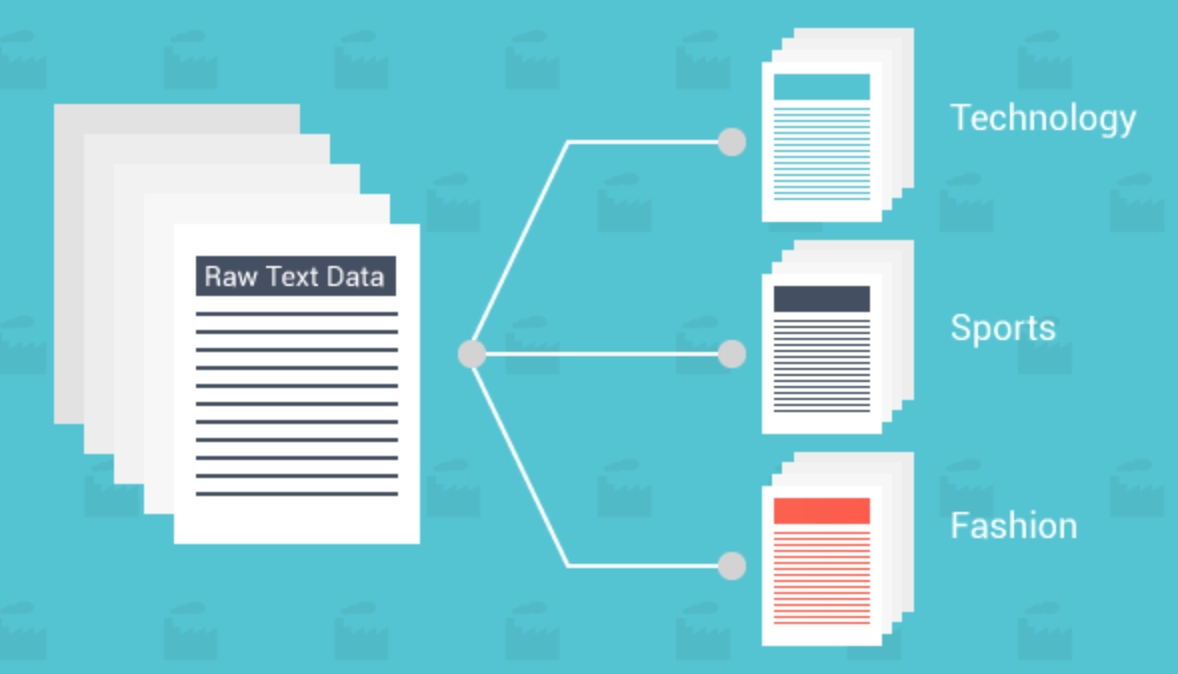
\includegraphics[width=\linewidth]{文本分类.png}
    \caption{文本分类}
  \end{subfigure}
  \begin{subfigure}[b]{0.4\linewidth}
    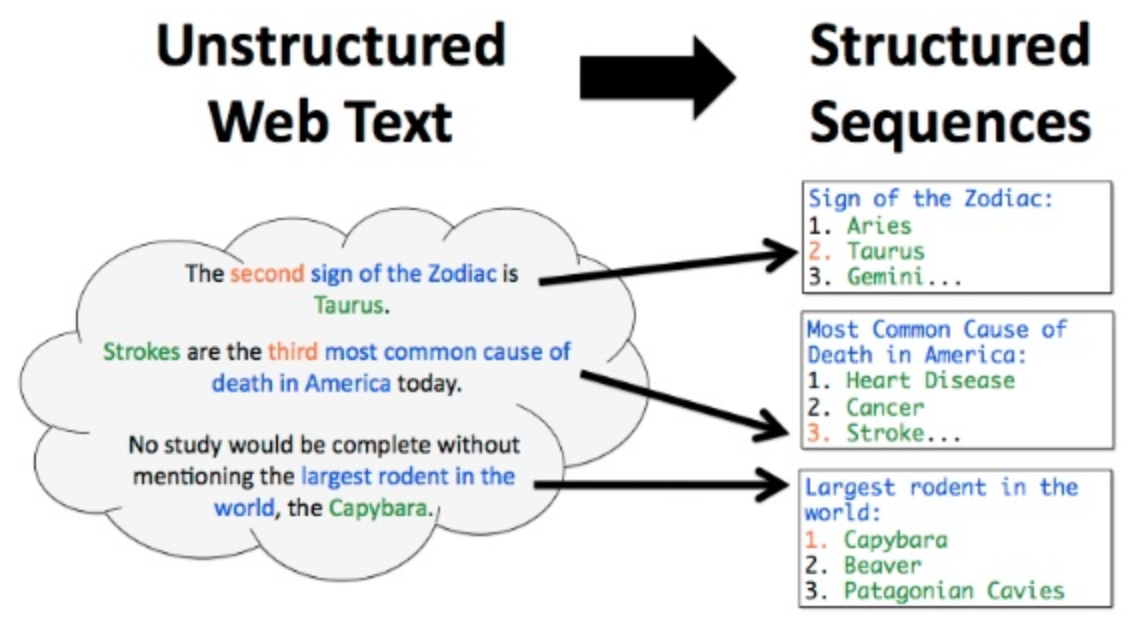
\includegraphics[width=\linewidth]{信息抽取.png}
    \caption{信息抽取}
  \end{subfigure}
  \begin{subfigure}[b]{0.4\linewidth}
    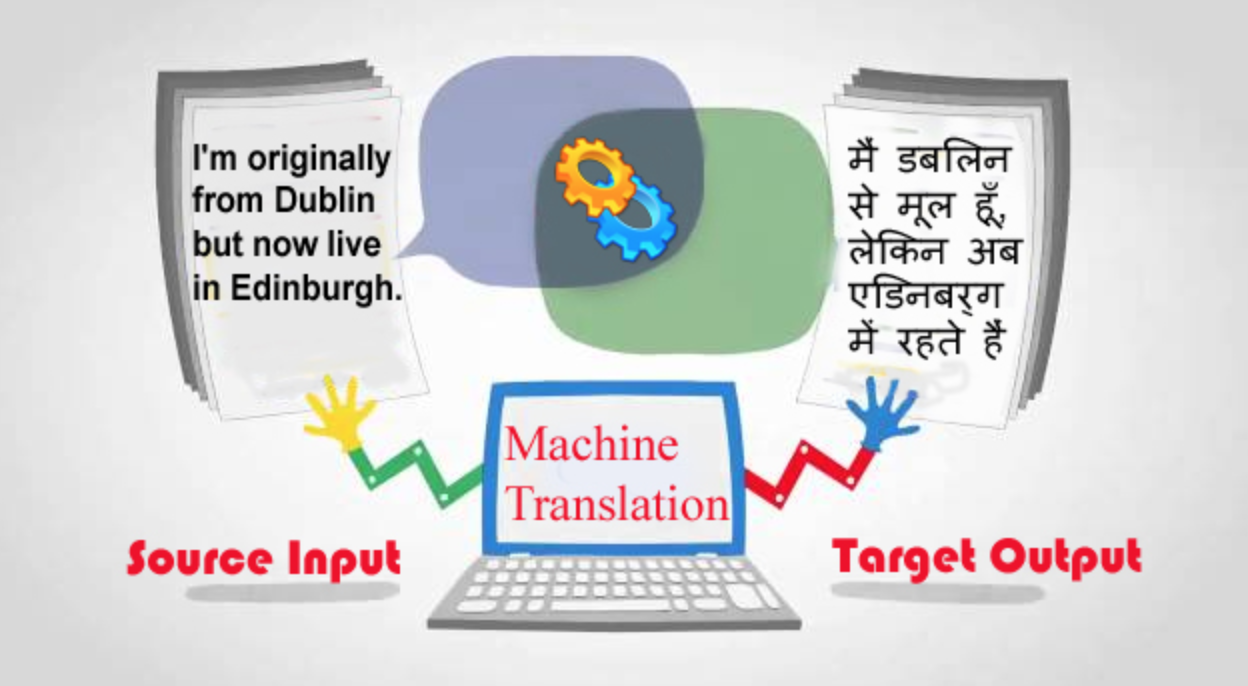
\includegraphics[width=\linewidth]{机器翻译.png}
      \caption{机器翻译}
  \end{subfigure}
  \begin{subfigure}[b]{0.4\linewidth}
    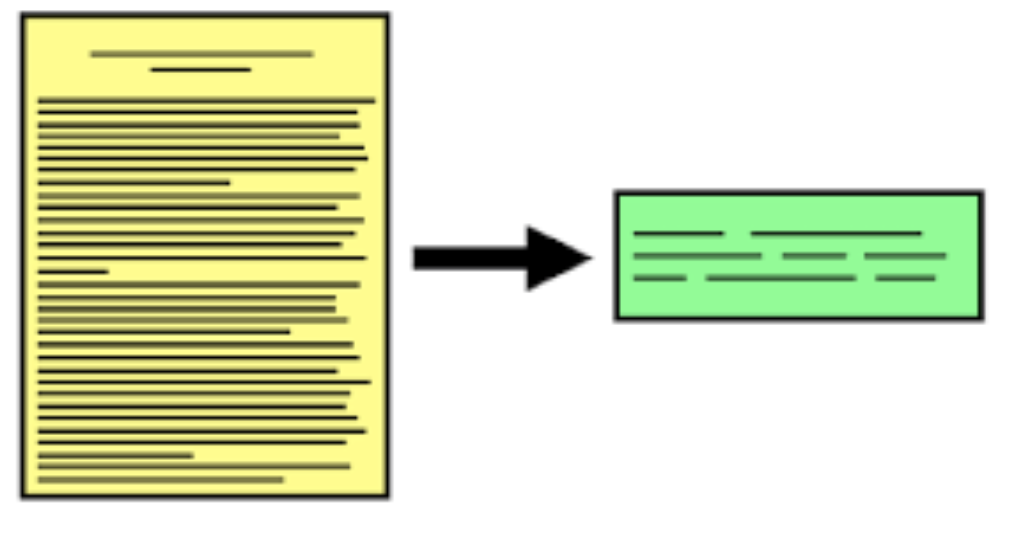
\includegraphics[width=\linewidth]{自动摘要.png}
    \caption{自动摘要}
  \end{subfigure}
  \begin{subfigure}[b]{0.4\linewidth}
    
\includegraphics[width=\linewidth]{问答系统.png}
    \caption{问答系统}
  \end{subfigure}
  \begin{subfigure}[b]{0.4\linewidth}
      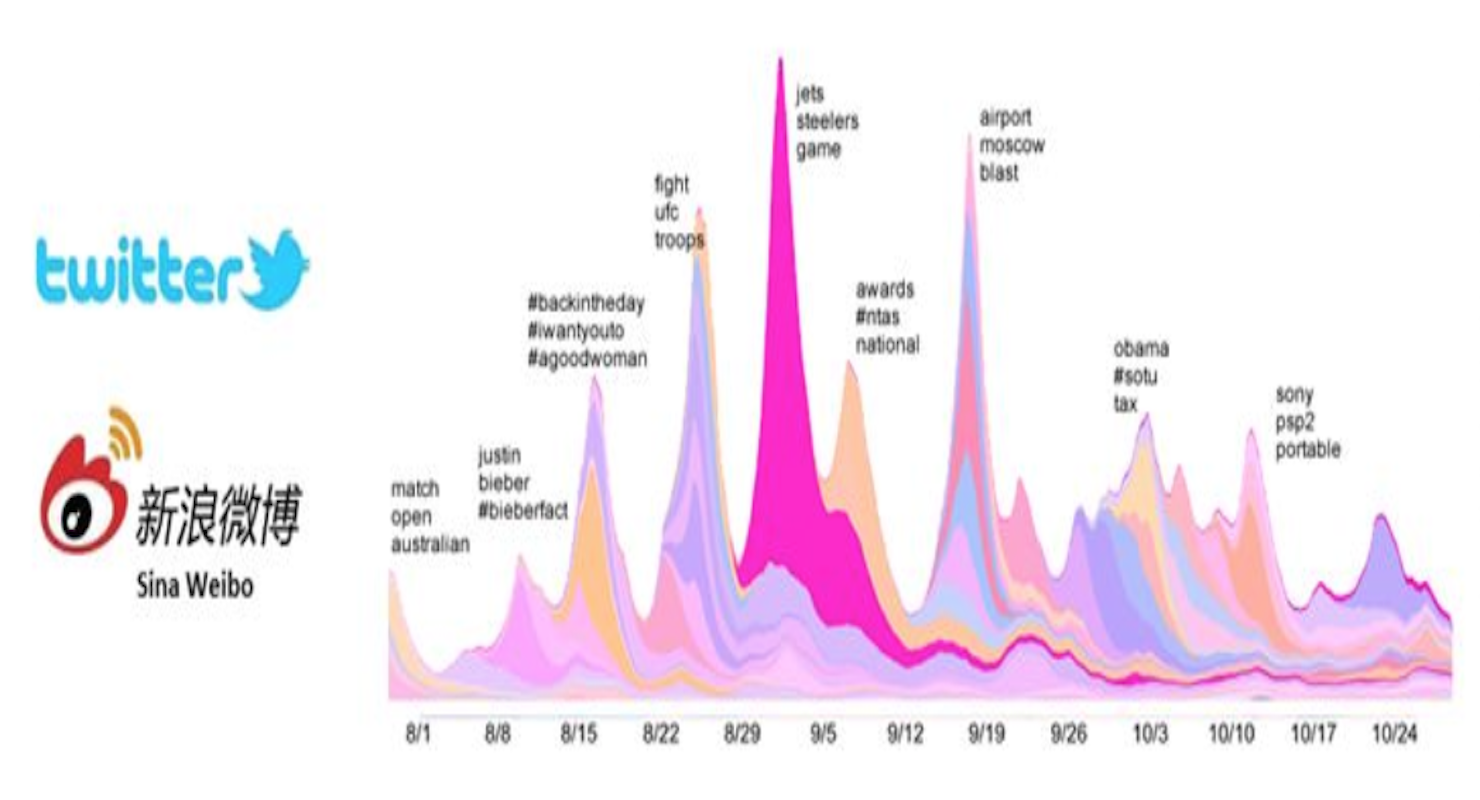
\includegraphics[width=\linewidth]{舆情分析.png}
      \caption{舆情分析}
  \end{subfigure}
  \caption{文本理解的相关应用}
\end{figure}


所以对文本理解技术的研究必然可以推动NLP领域的发展,从而直接或间接推动这些应用的性能和实用性的提高,具有重要的研究意义和价值.

\section{文本理解研究的发展与现状}
\subsection{文本理解的早期发展}
文本内容理解的研究最早是从1954年的Georgetown大学的机器翻译系统\cite{SlocumMachine}研发开始的,
但是一开始是通过制定规则的语法入手,所以在系统构建上有很大的局限性,带来了翻译质量的低劣.
随着研究的深入,基于规则的思路面临越来越多的困难.1966年,美国科学院语言自动处理委员会(Automatic Language Processing Advisory Committee)
公布了一个题为《语言与机器》的报告(简称ALPAC报告\cite{Pardelli2008From}),该报告全面否定了机器翻译的可行性,并建议停止对机器翻译项目的资金支持.

此后一段时间对与机器翻译的研究跌倒了谷底,但是研究者仍然坚持对计算语言的理论进行研究,并产生了很多非常重要的研究成果,
比如在句法研究上1969年J.Earley提出的Earley句法分析算法\cite{Earley1970An}等,在语义分析上1966年C.J.Filmore提出的格语法等.


直到80年代后期,人们通过构建语料库,把基于语料库的统计方法引入到自然语言处理中,
尤其是把已经在语音识别中取得成功的隐马尔可夫模型(Hidden Markov Model,HMM)\cite{Bangalore2010Sequence}引入到自然语言处理上,
起到了推波助澜的效果,很多人开始通过在大规模语料库上运用统计机器学习方法,并量化的评价和比较各种评价方法的性能.


此后自然语言处理领域的研究从基于规则方法转到基于统计的方法.

\subsection{文本理解的研究现状}
Ruhi Sarikaya在2011年指出一个自然语言理解系统包括3个任务:
领域识别(domain detection),意图分类(intent determination)和属性抽取(slot filling)\cite{Sarikaya2011Deep},
它们是一个连续的过程,首先识别文本领域,之后对用户意图进行分类,最后实现属性抽取.

从技术上讲,领域识别和意图分类是一个分类问题,通常使用传统的分类算法实现,
如2003年Haffner等人\cite{Bangalore2010Sequence}提出的支持向量机(Support Vector Machine,SVM)和
Chelba等人\cite{Chen2011Maximum}提出的最大熵算法(Maximum Entropy Classifier).
2014年Chen等人\cite{Ravuri2015Recurrent}提出也可以采用神经网络(Neural Network Classifier)来解决该问题.
而对于属性抽取则可以认为是一个序列标注问题,可以运用隐马尔可夫模型
和条件随机场(Conditional Random Field,CRF) 模型解决.

随着深度学习的发展,神经网络模型也被应用来处理领域识别和意图分类问题.
值得注意的是,Ravuri 和Stolcke 在2015年提出可采用循环神经网络(Recurrent Neural Network,RNN)来解决意图分类问题.
而对于属性抽取,可通过深度学习来提取特征并与传统的CRF相结合.Mesnil也尝试使用RNN进行序列标注以实现属性抽取\cite{Mesnil2013Investigation}.

循环神经网络经过实验证明在对序列化建模上效果显著,能够利用和记忆上下文信息,在几乎所有的NLP任务上都有很好的表现.
但是循环神经网络在反向传播求解的过程中会出现梯度消失和梯度爆炸的问题,所以对于长文本建模效果不佳.
后期提出的长短期记忆网络\cite{Graves2012Long}(Long Short-Term Memory,LSTM),通过在隐藏层设置3个“门”的结构,选择性的记忆和忘记,有效的解决了长文本建模的问题.
后来在此基础上有演化出许多改进的模型,比如树结构的长短期记忆网络\cite{Tai2015Improved}(Tree-LSTM),双向的长短期记忆网络\cite{Bahdanau2014Neural}(Bi-LSTM),
用来解决不同场景下的序列建模,如文本分类,中文分词,语义解析等.

目前以RNN为代表的深度学习模型已经成为了自然语言理解研究的主流方法.

但是上述研究均需要大量训练数据,并且一切都处于深度神经网络的黑盒中,使整个模型缺乏必要的直观性和鲁棒性.
而且最重要的是这种模型忽略了句子中的结构信息及语言学知识,而这些知识是可以用来辅助提升模型的,比如对于训练语料库中未出现的句子的词序列标注.

因此将语言的先验知识融入深度学习可以提高框架的可解释性和鲁棒性,将是 NLP 未来发展的重要方向.



\section{论文主要工作和贡献}
本文围绕研究将语言中的先验知识与深度学习模型进行有机融合,提出了融合依存句法结构的深度神经网络,并基于文本分类任务,研究融合模型的效果.
具体来说,本文的研究内容可以归纳为以下几个方面.

(1)通过斯坦福句法分析工具,构建文本的依存句法树,解析出子文本结构.

(2)研究和复现传统的RNN、LSTM等深度神经网络模型,并在LSTM模型的基础上融合依存句法信息,构建融合模型.

(3)研究了融合模型在不同规模数据集上表现和对通过可视化文本重要程度研究模型的可解释性.

(3)研究了文本结构的Attention机制和融合方式对模型效果的影响,并选择最佳的Attention和融合方式.

\section{论文结构安排}
本论文总共分为五个部分,各章节具体安排如下:

(1)第一章为绪论,首先介绍了文本理解的研究背景及意义,然后介绍了该领域的研究发展和 现状,并且简单描述了本文的研究内容,最后给出了全文的结构安排.

(2)第二章为基于深度学习的文本理解,
包括Word Embedding的文本表示方法,RNN、LSTM深度学习模型的介绍
以及基于深度学习的依存句法分析.

(3)第三章为融合句法结构树的深度神经网络模型,详
细介绍了融合模型的整体架构和每个模块的细节.

(4)第四章为实验部分,基于语料库AGNews,设计了融合模型和其他传统模型的对照实验,
并对不同的数据集、Attention方式、融合方式进行了深入的实验和分析.

(5)第五章为结论与展望,对本文主要工作进行了总结,对存在的不足进行了展望.


\chapter{基于深度学习的文本理解方法}
\section{文本的词向量表示方法}
自然语言处理领域最小的单元就是词语,通过词语构成句子,再有句子构成篇章.
所以为了让计算机能够处理文本首要任务就是对词语进行表示.
好的文本表示能够更加真是的反应文本的内容,对于不同的内容有更好的区分能力.

现在主流的表示方法是基于词向量(word embedding)的文本表示.
通过词向量可以讲词转化成稠密向量,对于相似的词,对应的词向量也相近.
这种表示方法又可以分为独热表示(one-hot representation)和分布式表示(distributed representation).

\subsection{独热表示}
用词向量表示文本,独热表示是一种最直接也是最简单的表示方法.
具体来说,每个词都表示成一个$n$维的向量,这里$n$为语料库中词表的大小.
假设某个单词在词表中的位置是$k$,那么这个单词的词向量只有位置$k$是1,
其他位置均是0.

比如有一个句子“我喜欢音乐,尤其是摇滚和嘻哈.”
如果整个语料库中就仅有这一个句子,这个句子分词后有8个不重复的单词,所以每个单词都可以表示为一个8维的向量,如下表所示.

\begin{table}[h!]
  \centering
  \begin{tabular}{cccccccc}
    \toprule
    \textbf{我} & \textbf{喜欢} & \textbf{音乐} & \textbf{尤其} & \textbf{是} & \textbf{摇滚}  & \textbf{和} & \textbf{嘻哈}  \\
    \midrule
    1 & 0 & 0 & 0 & 0 & 0 & 0 & 0 \\
    0 & 1 & 0 & 0 & 0 & 0 & 0 & 0 \\
    0 & 0 & 1 & 0 & 0 & 0 & 0 & 0 \\
    0 & 0 & 0 & 1 & 0 & 0 & 0 & 0 \\
    0 & 0 & 0 & 0 & 1 & 0 & 0 & 0 \\
    0 & 0 & 0 & 0 & 0 & 1 & 0 & 0 \\
    0 & 0 & 0 & 0 & 0 & 0 & 1 & 0 \\
    0 & 0 & 0 & 0 & 0 & 0 & 0 & 1 \\
    \bottomrule
  \end{tabular}
  \caption{8维独热词向量表示}\label{table:3t1}
\end{table}

这种表示方案如果采用稀疏方式存储,会是非常的简洁:也就是给每个词分配一个数字ID.
比如刚才的例子中,音乐记为2,摇滚记为5(从0开始记),如果要编程实现的话,用Hash表给每个词分配一个编号即可.
这么简洁的表示方法配合上最大熵、SVM、CRF等算法已经很好地完成了NLP领域的各种主流任务了.

但是这种表示方法也存在一个重要的问题就是“词汇鸿沟”现象:任意两个词之间都是孤立的,词向量之间都是正交.
光从两个向量中看不出两个词是否有关系,比如例子中的音乐和摇滚在语义上是相关的,但这种相关性无法从词向量上体现出来.

\subsection{分布式表示}
为了解决独热法无法体现语义的问题,Hinton等人\cite{Rumelhart1986Learning}在1986年提出了一种新的表示方法:Distributed representation,也就是“分布式表示”.
基本思想是通过训练将每个词映射成$K$维实数向量($K$一般为模型中的超参数),通过词之间的距离(比如 cosine 相似度、欧氏距离等)来判断它们之间的语义相似度.

2003年Bengio\cite{Turian2010Word}提出了一种经典的三层的神经网络“输入层-隐层-输出层”模型来训练词向量.
其核心思想是:一个给定单词的意思是由它的上下文确定的.
通过将被预测词的前$n$个词连接后作为神经网络的输入项,最后通过softmax层计算得到改词的词向量表示.
这种训练得到的词向量有很强的语义相关,
例如,$V(\mbox{意大利})-V(\mbox{罗马})+V(\mbox{巴黎}) = V(\mbox{法国})$,
类似的,$V(\mbox{国王})-V(\mbox{男人})+V(\mbox{女人})=V(\mbox{女王})$.
这样的结果非常振奋人心,但是这个算法对计算要求很高,训练效率较低.

2013年Google的Mikolov等人提出了Word2vec工具包\cite{Mikolov2013Distributed},里面包括了两种新的词向量模型:
CBOW(continuous bag of words)模型:给定上下文次,预测是否是中心词
和skip-gram模型:给定中间词,预测是否是上下文词.
工具包中还包括了两种高效训练的方法:负采样(negative sampling)和层序softmax(hierarchical softmax).
Word2vec大受欢迎的原因正是其高效性,Mikolov在论文中指出,一个优化的单机版本一天可训练上千亿词.

\begin{figure}[h!]
  \centering
  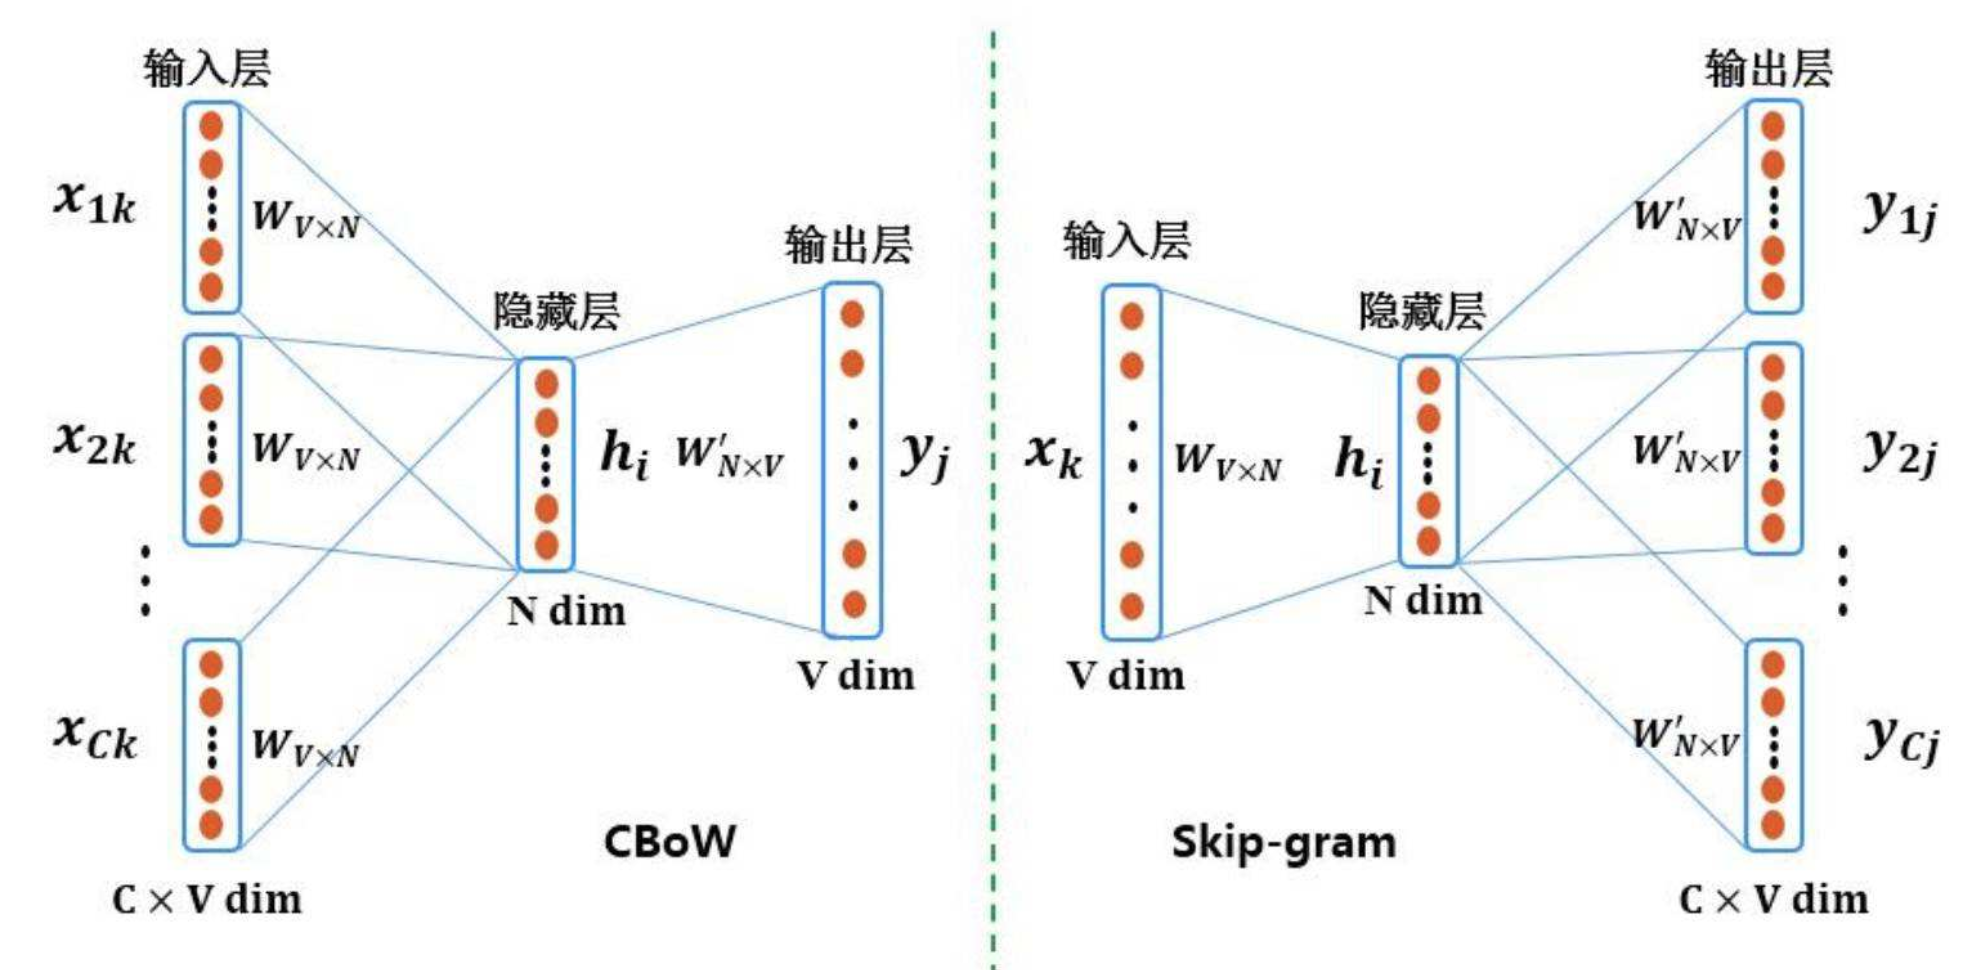
\includegraphics[width=0.6\linewidth]{CBOW-skip-gram.png}
  \caption{CBOW和skip-grams模型图示}
\end{figure}

具体来说,遍历文本中的每一个位置,包括一个中心词$c$和上下文单词$o$,通过词向量的$c$与$o$的相似度来计算$o$是$c$上下文的可能性,
通过调整词向量使得全局可能性达到最大.对于每个位置$t$,中心单词为$w_{t}$,窗口大小为$m$,那么全局可能性为:

\begin{equation}
  L(\theta) = \prod_{t=1}^{T} \prod_{-m \le j \le m ;j \neq m} P(w_{t+j}|w_{t},\theta)
\end{equation}

所以损失函数可以写成:
\begin{equation}
  J(\theta) = -\frac{1}{T}logL(\theta) = -\frac{1}{T} \sum_{t=1}^{T} \sum_{-m \le j \le m ;j \neq m} log P(w_{t+j}|w_{t},\theta)
\end{equation}

其中概率$P$通过$softmax$函数计算,采用梯度下降算法训练参数.

\subsection{GloVe模型}
Word2vec是基于局部上下文进行词向量训练的,所以并没有考虑到全局的信息.
2014年斯坦福大学的Jeffrey Penninngton等人\cite{Pennington2014Glove}提出了无监督学习的Glove(Global Vectors for Word Representation)模型.

其主要思想是以某个词的上下文窗口遍历整个语料库,统计窗口中词与词共同出现的次数,得倒整个语料库的词共现矩阵,
最后利用矩阵中的非零元素训练词向量.

设整个词共现矩阵为$X$,那么$X_{i}$为单词$w_{i}$上下文中所有出现词的总和,也就是矩阵第$i$行的和
,$X_{i,j}$表示单词$w_{i}$上下文中$w_{j}$出现的次数.那么单词$w_{j}$在$w_{i}$上下文中的概率为:

\begin{equation}
  P_{i,j} = P(w_{j}|w_{i}) = \frac{X_{i,j}}{X_{i}}
\end{equation}

两个词的共现概率就可以体现两个词的相关性.给定一个词$w_{k}$,通过计算$p_{ki}$ 与$p_{kj}$的比值,
来判断$w_{i}$和$w_{j}$哪一个与$w_{k}$更相关,如果比值大于1,则是单词$w_{i}$,反之就是单词$w_{j}$.
模型中词与词之间共现概率的比值可以最终转换成需要优化的目标函数:

\begin{equation}
  J = \sum_{i,j}^{N}f(X_{i,j})(v_{i}^{T}v_{j}+b_{i}+b_{j}-log(X_{i,j}))^2
\end{equation}

其中$v_{i}$,$v_{j}$是单词$i$和单词$j$的词向量,
$b_{i}$,$b_{j}$是两个标量,作者定义的偏差项,
$N$是词汇表的大小,共现矩阵维度为$N*N$,$f$是权重函数,需要满足一定的非递减性,
来保证对低频词共现组合不会赋值很大,所以一般$f(X_{i,j})$定义为:

\begin{equation}
  f(x) = 
  \left\{
    \begin{array}{lr}
      (x/x_{max})^{\alpha}, & x<x_{max} \\
      1, & x \ge x_{max} 
    \end{array}
    \right.
\end{equation}

其中,$\alpha$一般取$0.75$,$x_{max}$则根据语料库的实际情况而定.


\section{NLP领域的深度学习模型}
神经网络模型具备强大的学习能力和拟合能力,在图像,音频,NLP等诸多领域取得了非常好的效果.
NLP领域应用最为广泛的深度学习模型就是循环神经网络RNN和长短期记忆网络LSTM.

\subsection{循环神经网络}
传统的神经网络并不能做到持续记忆,这也应该是传统神经网络的一个缺陷.
如果让神经网络对电影中每个时间点的事件进行分类,很明显,传统神经网络不能使用前一个事件去推理下一个事件.
循环神经网络RNN的出现很好的解决了对序列数据建模的问题.

RNN之所以称为循环神经网路,是因为一个序列当前的输出与前面的输出有关.
具体的表现形式为网络会对前面的信息进行记忆并应用于当前输出的计算中,
即隐藏层之间的节点不再无连接而是有连接的,
也就是说隐藏层的输入不仅包括输入层的输出还包括上一时刻隐藏层的输出.
下图是一个典型的RNN结构图:

\begin{figure}[h!]
  \centering
  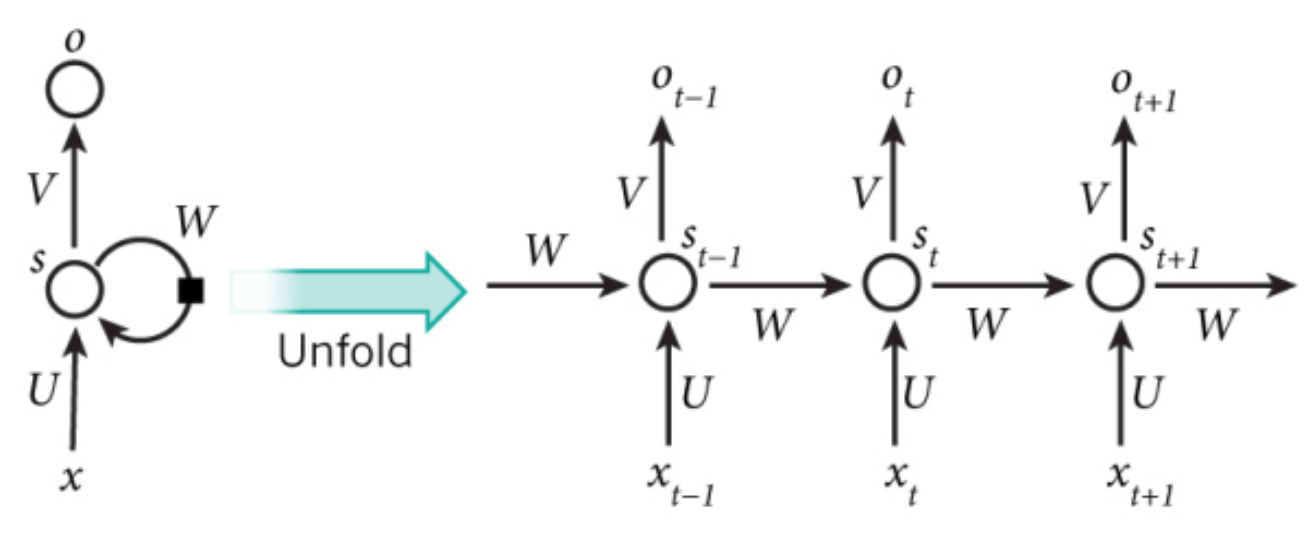
\includegraphics[width=0.6\linewidth]{RNN.png}
  \caption{RNN结构图}
\end{figure}

如图所示,把循环神经网络进行展开成一个全神经网络.
例如,对一个包含3个单词的语句,那么展开的网络便是一个有3层神经网络,每一层代表一个单词.
其中$x_{t}$表示第$t$步的输入,$s_{t}$为隐藏层的第$t$步的状态,它是网络的记忆单元.
$s_{t}$根据当前输入层的输出与上一步隐藏层的状态进行计算,$o_{t}$是第t步的输出.

\begin{equation}
  \left\{
  \begin{array}{l}
    s_{t} = f(U*x_{t}+W*s_{t-1}) \\
    o_{t} = softmax(V*s_{t})
  \end{array}
  \right.
\end{equation}

上式中的$f$表示非线性的激活函数,如$tanh$,$ReLU$.
需要注意的是:在RNN中,每输入一步,每一层各自都共享参数$U$,$V$,$W$.
其反映着RNN中的每一步都在做相同的事,只是输入不同,
因此大大地降低了网络中需要学习的参数,对于RNN的训练同样是误差反向传播算法.

RNN有4种常见的架构,1 to N、N to 1、N to N和N to M,这4种架构基本可以满足常见的NLP应用.

\begin{figure}[h!]
  \centering
  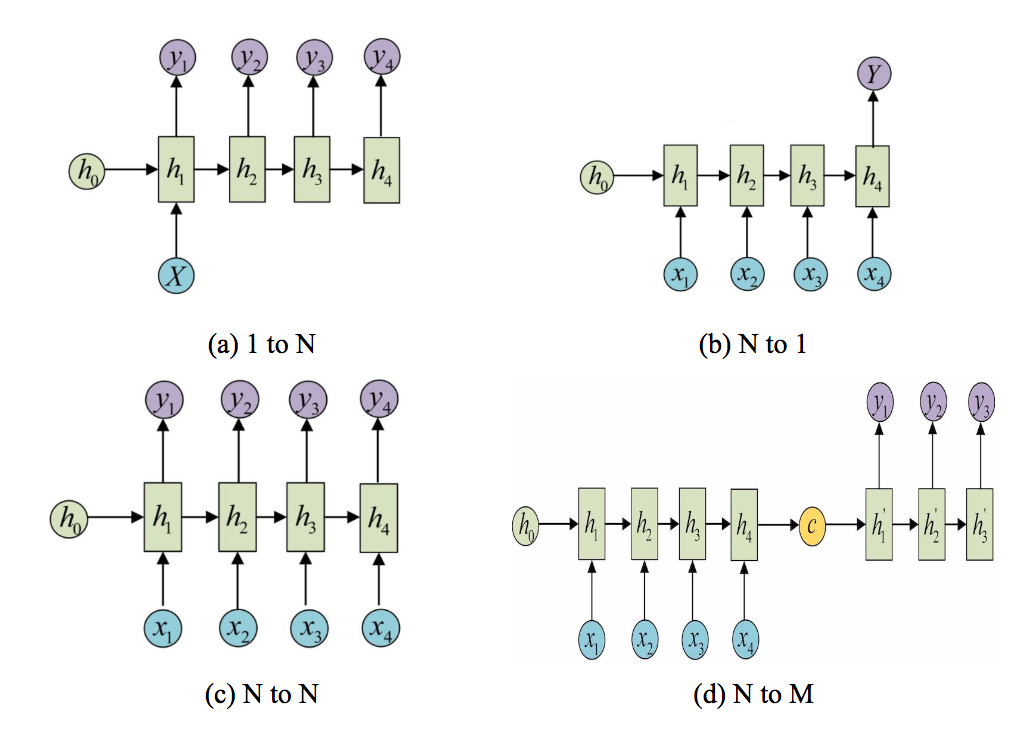
\includegraphics[width=0.65\linewidth]{4种架构.png}
  \caption{RNN4种架构}
\end{figure}

% \begin{figure}[h!]
%   \centering
%   \begin{subfigure}[b]{0.4\linewidth}
%     \includegraphics[width=\linewidth]{1ton.png}
%     \caption{1 to N}
%   \end{subfigure}
%   \begin{subfigure}[b]{0.4\linewidth}
%     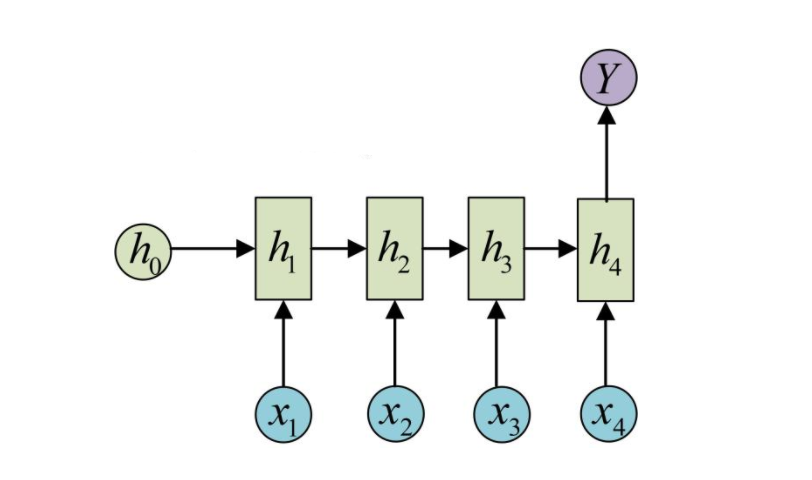
\includegraphics[width=\linewidth]{nto1.png}
%     \caption{N to 1}
%   \end{subfigure}
%   \begin{subfigure}[b]{0.4\linewidth}
%     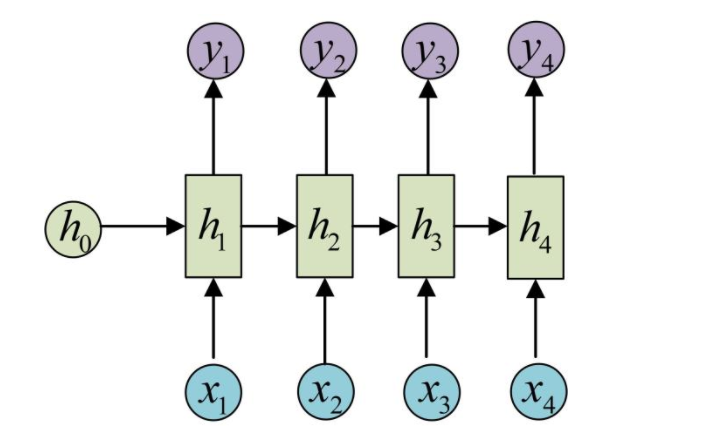
\includegraphics[width=\linewidth]{nton.png}
%       \caption{N to N}
%   \end{subfigure}
%   \begin{subfigure}[b]{0.4\linewidth}
%     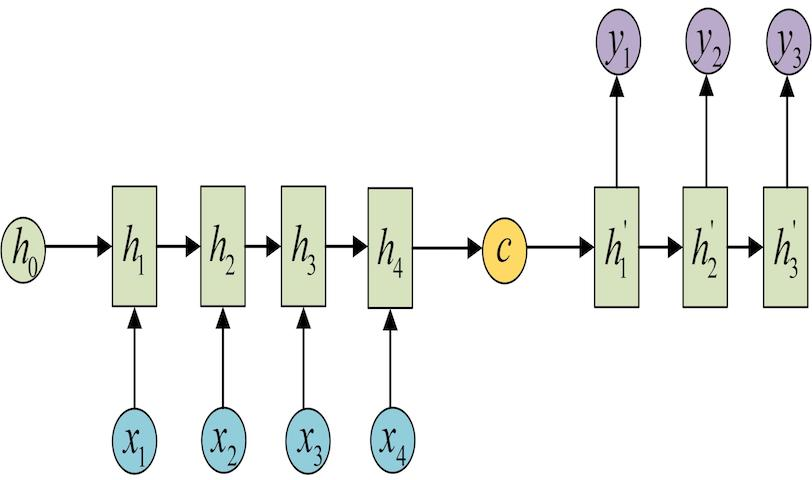
\includegraphics[width=\linewidth]{ntom.jpg}
%     \caption{N to M}
%   \end{subfigure}
%   \caption{RNN的4种常见的架构}
% \end{figure}


(1)1 to N:输入是一个值,输出是一个序列.比如图片标注,输出的X是图像的特征,而输出的y序列是一段句子,或者输入类别x,输出的y是该类别的一串文字.

(2)N to 1:输入是一个序列,输出是一个单独的值.这种结构通常用来处理序列分类问题.如输入一段文字判别它所属的类别,输入一个句子判断其情感倾向等.

(3)N to N:输入和输出是等长的序列.这种可以作为简单的Char RNN可以用来生成文章,诗歌,甚至是代码.

(4)N to M:这种结构又叫Encoder-Decoder模型,也可以称之为Seq2Seq模型.在实现问题中,我们遇到的大部分序列都是不等长的,如机器翻译中,源语言和目标语言的句子往往并没有相同的长度.
而Encoder-Decoder结构先将输入数据编码成一个上下文向量c,之后在通过这个上下文向量输出预测序列.

但是RNN在处理长期依赖(时间序列上距离较远的节点)时会遇到巨大的困难,
因为计算距离较远的节点之间的联系时会涉及雅可比矩阵的多次相乘,
这会带来梯度消失(经常发生)或者梯度膨胀(较少发生)的问题.

\subsection{长短期记忆网络}
为了解决RNN对长序列建模的困难,研究人员提出了许多解决办法,例如ESN(Echo State Network),
增加有漏单元(Leaky Units)等.
其中最成功应用最广泛的就是门限RNN(Gated RNN),而长短期记忆网络LSTM就是门限RNN中最著名的一种.

\begin{figure}[h!]
  \centering
  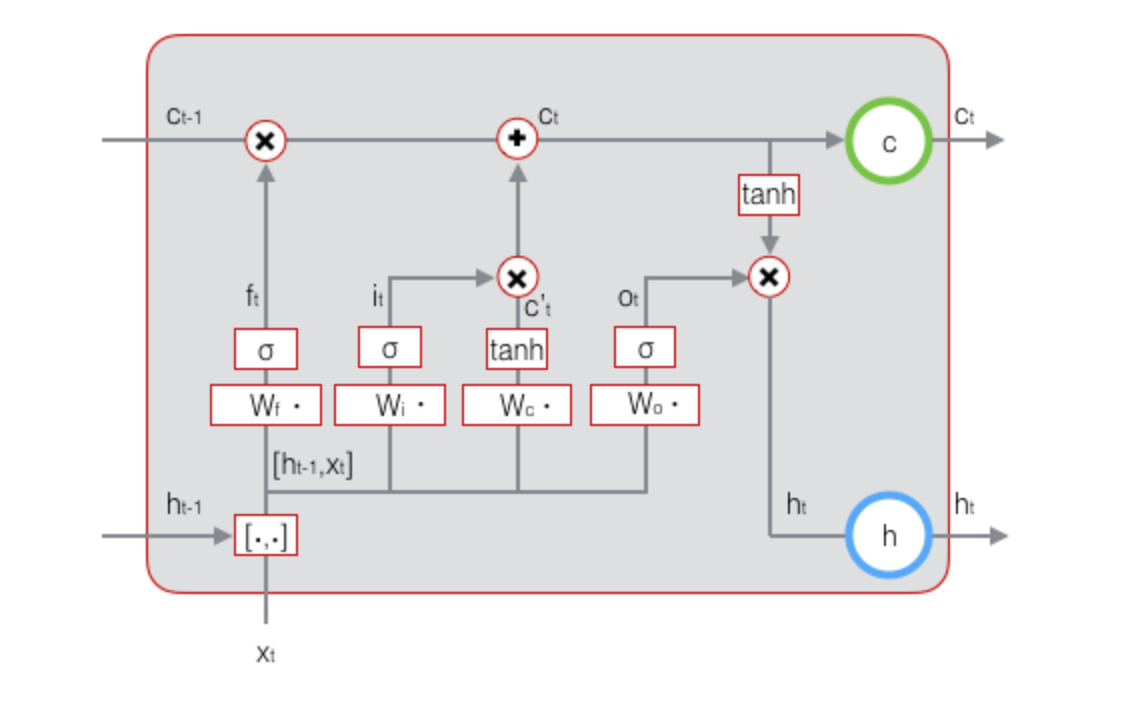
\includegraphics[width=0.6\linewidth]{LSTM.png}
  \caption{LSTM模型}
\end{figure}

如上图所示,LSTM一个单元通过输入门、遗忘门、输出门三个门来控制信息的流动,
其中输入门控制信息的流入,
遗忘门负责丢弃记忆细胞中的无用信息,
最后输出门控制信息的输出.
还有一个记忆细胞负责储存先前的信息和产生下一个输出.
对应的公式为:

\begin{equation}
  \left\{
  \begin{array}{l}
   i_{t} = \sigma(W^{xi}x_{t}+W^{hi}h_{t-1}+b_{i}) \\ 
   o_{t} = \sigma(W^{xo}x_{t}+W^{ho}h_{t-1}+b_{o}) \\ 
   f_{t} = \sigma(W^{xf}x_{t}+W^{hf}h_{t-1}+b_{f}) \\ 
   \widetilde{c}_{t} = \sigma(W^{xc}x_{t}+W^{hc}h_{t-1}+b_{c}) \\
   c_{t} = f_{t} \odot c_{t-1} + i_{t} \odot \widetilde{c}_{t} \\
   h_{t} = o_{t} \odot c_{t}
  \end{array}
  \right.
\end{equation}

式子中的$W$和$b$是模型参数,$i_{t}$,$o_{t}$,$f_{t}$对应$t$时刻的输入门,输出门和遗忘门,
$\widetilde{c}_{t}$,表示遗忘细胞更新量,由输入门,遗忘门,上一个时刻的记忆细胞,和当前记忆细胞的更新量,共同计算当前的记忆细胞值.
然后通过当前的记忆细胞和输出门计算当前时刻的隐层输出$h_{t}$.

显然LSTM单元可以无缝的替换传统的RNN单元,
所以LSTM也有4种架构,
采用RNN模型的应用几乎都可以很方便的替换成LSTM模型.
但是这类模型,并没有运用到语言本身句法结构中的信息,模型处于黑盒之中,缺乏必要的直观性和鲁棒性.

\section{基于深度学习的依存句法分析}
\subsection{依存句法的概念}
1960年基于当时机器翻译的特点,美国语言学家D.GHays提出了依存句法的概念\cite{Hays1960Grouping}.
这里的“依存”是词与词之间的支配和被配置关系,并且这样的关系是有方向性的,不是对等的.
在依存结构图中用带有方向的弧表示支配和被支配关系.
也即指出了词语之间在句法上的搭配关系,这种搭配关系是和语义相关联的.
比如“I shot an elephant in my pajamas.”的依存句法结构如下图所示.

\begin{figure}[h!]
  \centering
  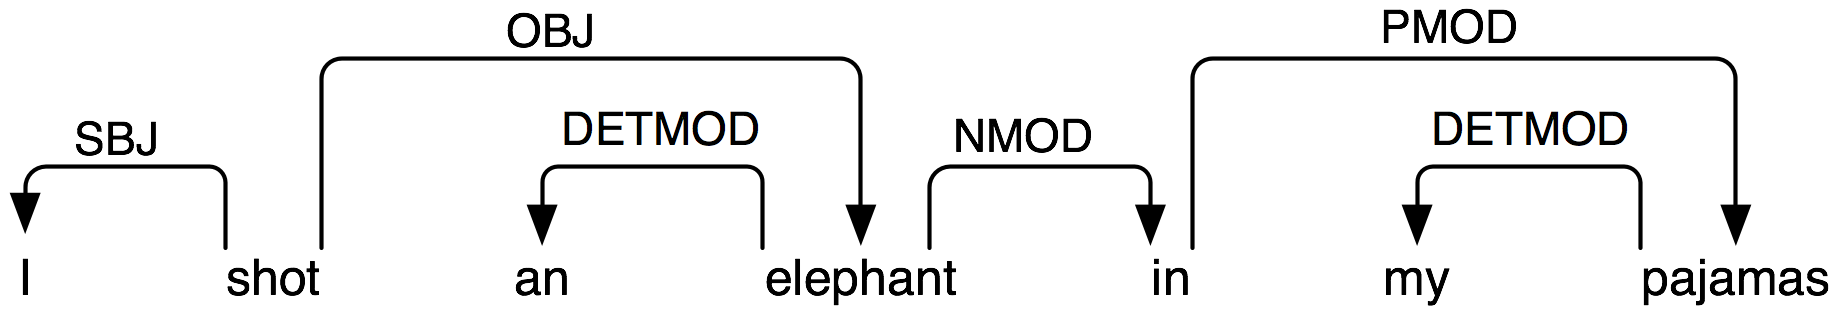
\includegraphics[width=0.7\linewidth]{依存句法.png}
  \caption{依存句法示意图}
\end{figure}

随着句法理论的发展计算机语言学家罗宾森总结了依存语法的五条定理:

(1)一个句子中存在一个成分称之为根(root),这个成分不依赖于其它成分.

(2)其它成分直接依存于某一成分.

(3)任何一个成分都不能依存与两个或两个以上的成分.

(4)如果A成分直接依存于B成分,而C成分在句中位于A和B之间,那么C或者直接依存于B,或者直接依存于A和B之间的某一成分.

(5)中心词两边的成分不存在依存关系.

所以一个句法结构中只有一个根节点,并且可以用树来表示整个结构,如下图所示,树中层次低的节点依存层次高的节点,
也就是树中的父节点支配子节点.

\begin{figure}[h!]
  \centering
  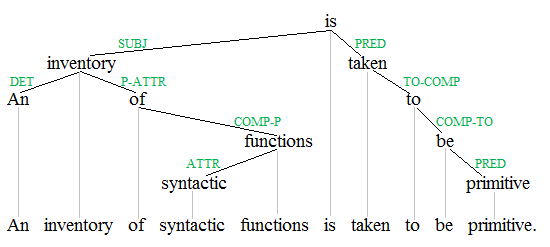
\includegraphics[width=0.6\linewidth]{依存句法树.png}
  \caption{依存句法树示意图}
\end{figure}

句子成分中的支配和被支配的依存关系具有广泛的普遍性,
在词汇,短语,篇章等各级别的语言单位之间都存在.
所以依存句法反应了句子内部的词与词之间的语义修饰关系,
并且这种关系和词与词之间的位置关系是没有联系的,
所以直接体现了句子中蕴含的语言学知识,具有很大的利用价值.

\subsection{Stanford Parser}
Stanford Parser 是由斯坦福大学自然语言处理小组开发的开源句法分析器.
最新版的分析器是基于深度神经网络的,由Danqi在2014年提出并实现\cite{The}.

整个模型具体来说,首先先把每个单词表示成一个$d$维的向量$e_{i}^{w} \in \mathbb{R}$,
所以整个词向量矩阵就是$E^{w} \in \mathbb{R}^{d*N_{w}}$,
这里的$N_{w}$表示词典的大小.
同时吧POS标签和弧形标签映射成一个$d$维的向量,
$e^{t}_{i}$,$e^{l}_{j}$分别表示第$i$个POS标签和第$j$个弧标签,
所以整体上$E^{t} \in \mathbb{R}^{d*N_{t}}$,$E^{l} \in \mathbb{R}^{d*N_{l}}$,
这里的$N_{t}$表示POS标签数量,$N_{l}$表示弧度标签数量.
通过建立一个标准的神经网络,有一个隐藏层,把$(word,POS,arc)$的组合
作为神经网络的输入,并且把输入的3次方映射成隐藏层,最后通过一个softmax函数.
网络的结构如下图所示.


\begin{figure}[h!]
  \centering
  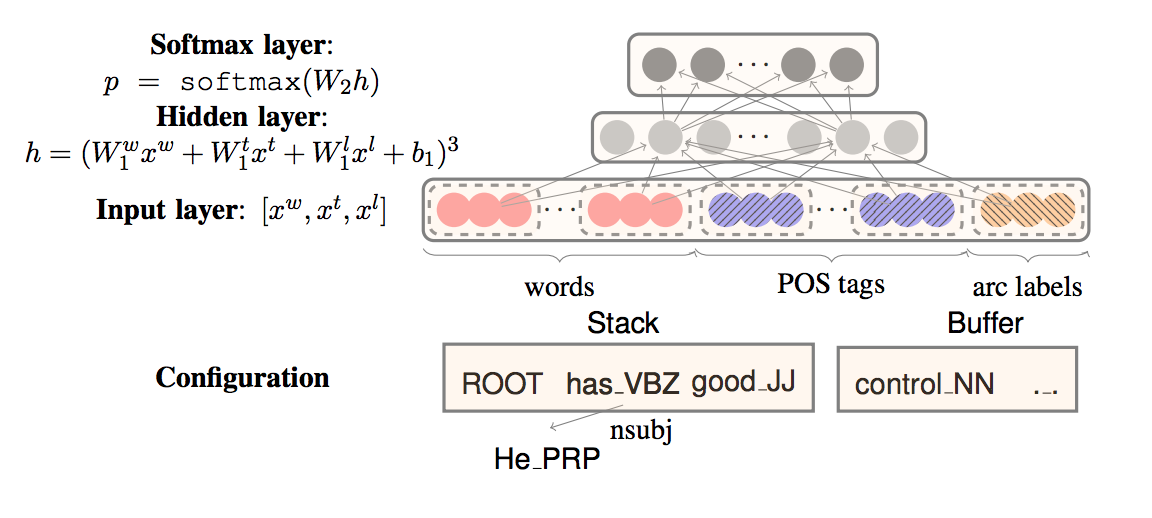
\includegraphics[width=0.85\linewidth]{斯坦福句法分析模型.png}
  \caption{斯坦福句法分析模型}
\end{figure}

这个模型提出后,在CoNLL依存句法数据集上一直稳居第一名.具体来说Stanford parser有下面几大优点:

(1)既是一个高度优化的概率上下文无关文法和词汇化依存分析器,也是一个词汇化上下文无关文法分析器.

(2)基于权威可靠的宾州树库(Penn Treebank)作为分析器的训练数据,目前已面向英文、中文、德文、阿拉伯文、意大利文、保加利亚文、葡萄牙文等语种提供句法分析功能.

(3)提供了多样化的分析输出形式,除句法分析树输出外,还支持分词和词性标注文本输出、短语结构树输出、斯坦福依存关系输出等。

(4)分析器内置了分词工具、词性标注工具、基于自定义树库的分析器训练工具等句法分析辅助程序.

(5)通过设置不同的运行参数,可实现句法分析模型选择、自定义词性标记集、文本编码设置和转换、语法关系导入和导出等功能的定制.

在使用上Stanford Parser是给予Java语言开发的,也提供了多个语言的变成接口,
并且还可以以服务的方式运行,提供API调用.
目前已经集成进了Stanford CoreNLP工具包中.



\chapter{融合句法结构的深度神经网络模型}
本章节详细介绍提出的融合句法结构的深度神经网络模型(下文简称:融合模型).
该模型是将蕴含语言学知识的依存句法结构信息融合到传统的LSTM模型中,
以提升文本理解的效果.
\section{模型设计}
这个部分讲说明如何对文本内容和语言学知识进行向量化的编码,
并着重说明融合模型的架构,详细说明各个模块的运作方式.
\subsection{词向量设计}
有两个词向量的设计工作,第一是将文本的向量化,第二是将依存句法结构向量化.

对于第一个文本的向量化,可以采用先前介绍的Glove模型来训练词向量,
也可以直接从官网https://nlp.stanford.edu/projects/glove/上下载已经训练好的词向量,
词向量的维度可以选择,这些词向量是通过英文维基百科训练的,包括50,100,200,300维等.
设每个单词表示成一个$d$维的向量$e_{i}^{w} \in \mathbb{R}$,所以一段文本可以表示为
$E^{w} \in \mathbb{R}^{d*N_{w}}$,其中$N_{w}$表示这段文本的长度.

对于第二个依存句法结构的向量化,首先通过依存句法分析工具生成依存句法树.
这样可以获得依存句法树根节点到叶子节点的形成的子结构.
比如,对于句子“show me the flights from seattle to san francisco.”
可以获得的子结构如下图所示,

\begin{figure}[h!]
  \centering
  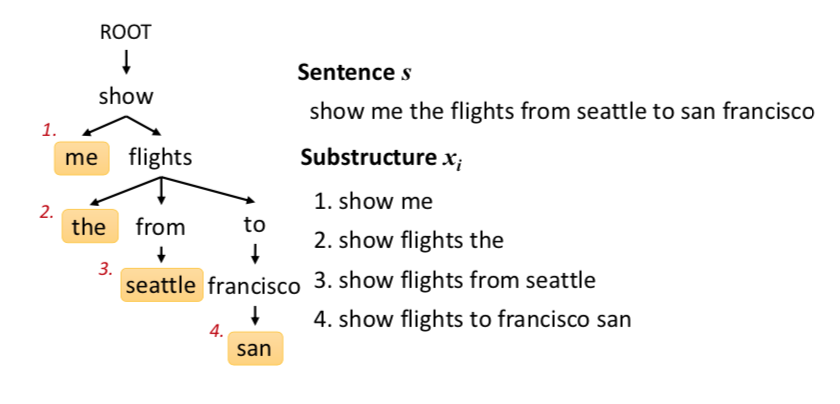
\includegraphics[width=0.8\linewidth]{依存句法树举例.png}
  \caption{根据依存句法树获得子结构}
\end{figure}

这样上面图中的依存句法结构就可以通过这4个子串$x_{1},x_{2},x_{3},x_{4}$来表示,
事实上仅仅通过这4个子串就可以反过来推导出依存句法树,
所以依存句法树和其从根节点到叶子节点的子串是相互唯一确定的.

下面就可以对这4个子串进行向量化,每个单词依然表示成一个$d$维的向量,
那么一个子串$x_{i}$就可以表示为$E_{x_{i}} \in \mathbb{R}^{d*N_{x_{i}}}$,
这里$N_{x_{i}}$表示子串$x_{i}$的单词个数.
这里我们没有利用依存句法中的弧标签信息,因为这些信息并不是在所有的语料中都可以获取,所以不具备普适性.
值得注意的是所有子串的总数一定是小于文本中所有单词数量的,
因为子串是根据叶子节点获得的,非叶子节点就没有对应的子串,
这样也可以减少模型中的重复信息.

最后还需要说明一下,如何根据依存句法树中获得所有从根节点到叶子结点的子串,
事实上可以通过一个简单的递归算法解决,具体如下.

\begin{table}[h!]
  \centering
  \begin{tabular}{l}
    \toprule
    \textbf{递归获取依存句法树子串算法描述} \\
    \midrule
    (1)输入: 依存句法树Tree \\
    (2) 定义所有子串的列表$all\_substructures$,路径字符串$path$ \\
    (3) 定义递归函数$walk(node,path)$,$node$为当前节点 \\
    (3.1) 路径字符串加上当前节点的值 $path = path + node.value$ \\
    (3.2) 判断当前节点是不是叶子结点,如果是转到(3.3),如果不是转到(3.4)\\
    (3.3) 所有子串的列表加上当前的路径字符串,$all\_substructures.append(path)$ \\
    (3.4) 对该节点所有的子节点递归调用,$walk(node.childnode,path)$ \\
    (4)调用 $walk(Tree.root\_node,path)$ \\
    (5)输出所有子串的列表$all\_substructures$ \\
    \bottomrule
  \end{tabular}
  \caption{递归获取依存句法树子串算法描述}
\end{table}
通过上面的算法输入依存句法树就可以获取所有的子结构.

\subsection{模型架构}
融合句法结构的深度神经网络模型的整体架构如下图所示:
\begin{figure}[h!]
  \centering
  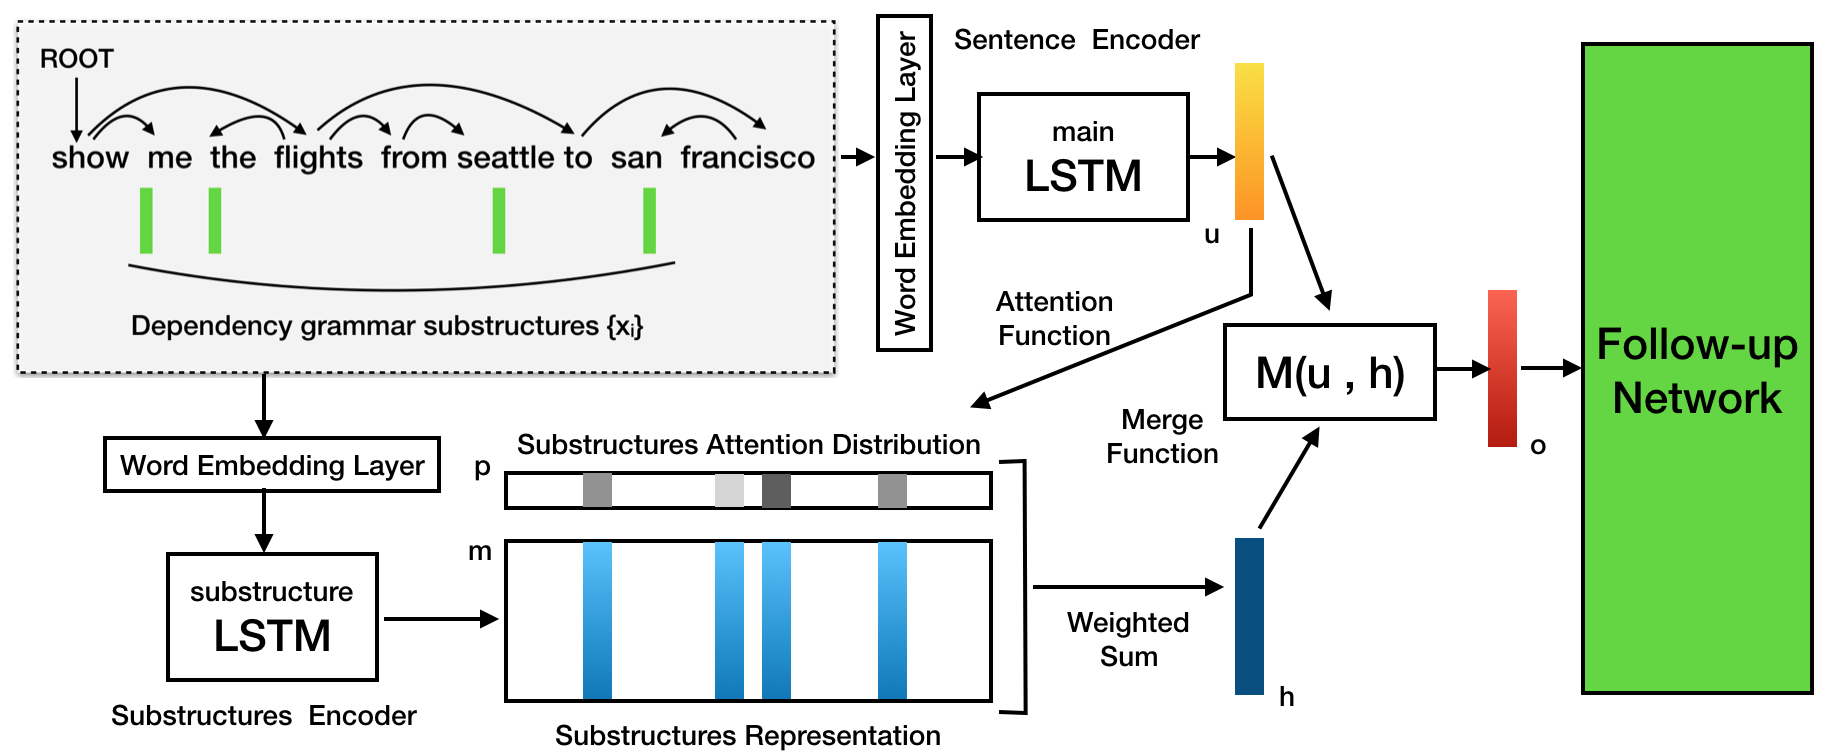
\includegraphics[width=0.95\linewidth]{model.png}
  \caption{融合句法结构的深度神经网络模型}
\end{figure}

整个模型图示从左向右看子结构句子和主文本句子分别通过两个LSTM模型,
将子结构输出的结果加权平均后与主文本句子的输出结果相融合,
得到一个最终的融合表示,最后将这个表示送入后续的神经网络中,
完成文本分类、机器翻译等文本理解的应用.下面对具体的阐述模型中的几个细节.

(1) 这里的词嵌入层直接采用Glove的词向量,只需要将单词与词向量进行一一映射即可.
词向量的维度$d$是模型的超参数.

(2)LSTM模块采用单层经典的LSTM模型即可,事实上在本模型中,LSTM可以看成一个编码器,
我们只取LSTM的最后一个隐藏层节点,因为LSTM具有记忆的功能,
所以最后一个节点可以认为是对整个输入文本的编码.
所以$x_{i}$被编码成$m_{i}$,整个文本句子$s$被编码成$u$,
其中$m_{i} \in \mathbb{R}^{H_{sub}}$ ,$H_{sub}$为子结构LSTM隐藏层节点个数,
$u \in \mathbb{R}^{H_{main}}$,$H_{main}$为主LSTM隐藏层节点个数.

\begin{equation}
\left\{
  \begin{array}{l}
   m_{i} = LSTM_{sub}(x_{i}) \\ 
   u = LSTM_{main}(s) \\ 
  \end{array}
  \right.
\end{equation}

LSTM的内部推倒可以见2.2.2小节,
下面通过一个图示来说明通过LSTM模型的过程,
一个子结构句子“show me the”通过LSTM,
并将最后一个隐藏层输出作为编码结果$m$.

\begin{figure}[h!]
  \centering
  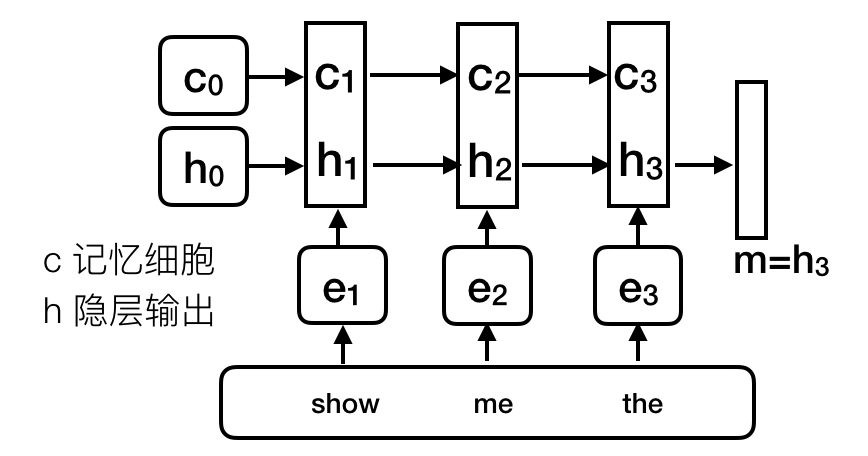
\includegraphics[width=0.5\linewidth]{LSTM具体.png}
  \caption{$x$通过LSTM编码得到$m$}
\end{figure}

(3)
通过Attention函数来计算整个句子的编码$u$和每一个子结构$m_{i}$的匹配程度.

具体可以分成两步,打分函数$Socre\_Function$和$softmax$函数,
首先通过打分函数计算相关性的评分,然后再通过sotfmax来计算匹配概率$p_{i}$,
这里的$p_{i}$就可以认为是每一个子结构对
理解这个文本的重要程度.

\begin{equation}
  \left\{
    \begin{array}{l}
     socore_{m_{i}} = Socre\_Function(u,m_{i}) \\ 
     p_{i} = softmax(socore_{m_{i}}) \\ 
     softmax(z_{i}) = \frac{e^{z_{i}}}{\sum_{j} e^{z_{j}}}
    \end{array}
  \right.
\end{equation}

这里的打分函数有多种表达形式,具体会在下一节中着重说明.

(4)
$h$是子结构加权平均的结构,可以用来表现句子依存句法结构的信息,
也就是说这个向量事实上代表了文本$s$的语言学知识.

\begin{equation}
  h = \sum_{i}(p_{i}m_{i})
\end{equation}

(5)
向量$o$是主文本LSTM输出$u$和文本子结构LSTM输出加权$h$融合的结果.
可以作为整个融合模型的输出,送入到后续的网络中.
\begin{equation}
  o = M(u,h)
\end{equation}

式子中的函数$M$是融合函数,有多种融合方式,具体会在后面的小节中着重说明.

(6)后续的网络,事实上可以接入任何形式的网络,完成众多不同的文本理解任务.
因为这个融合模型的初衷就是可以无缝替换原先的LSTM模型,所以融合模型的输入和输出,
与传统的LSTM模型的输入和输出是完全相同的,
不过融合模型的输出中附加了句法结构的语言学知识.

如后续网络接入情感分类(简化仅有两类情感)网络,如下图所示.
把融合网络的输出向量$o$,
接到一个全连接的神经网络中,网络为了简化,这里只有一层,也就是两个隐藏层节点,
后面再接一个softmax层,就可以获得这个文本两类情感的概率分别是多少,
取概率较高的类别作为最终的情感类别.
\begin{figure}[h!]
  \centering
  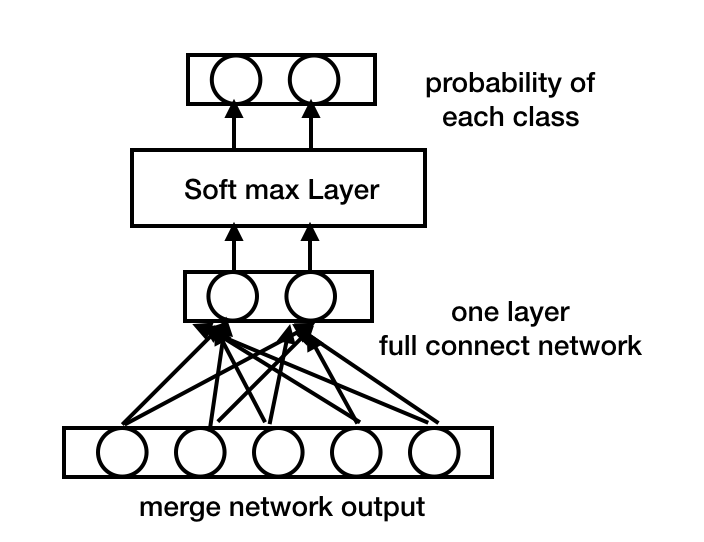
\includegraphics[width=0.5\linewidth]{二分类.png}
  \caption{后续接入情感分类网络}
\end{figure}

再如后续网络接入1toM网络,就可以实现一个机器翻译的网络,如下图所示.
把融合网络的输出向量$o$,接到到LSTM中,这样每个隐层的输出$y_{i}$,
就构成了一个序列的向量,进而把每个$y_{i}$映射成字符$w_{k}$,
这样取得了一连串的字符输出,可以作为一个简化的机器翻译网络.

\begin{figure}[h!]
  \centering
  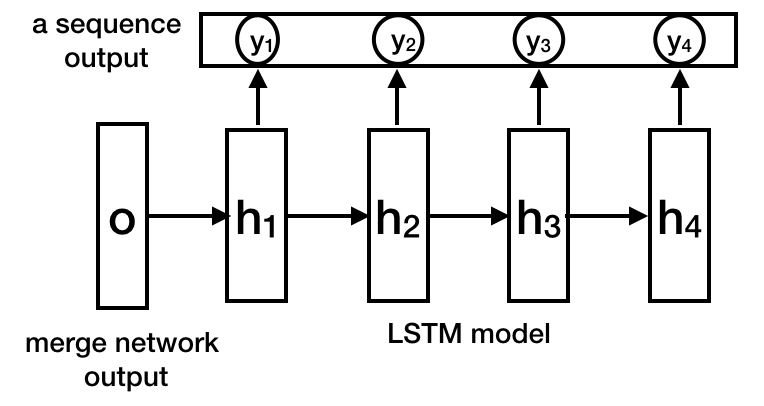
\includegraphics[width=0.5\linewidth]{机器翻译例子.png}
  \caption{后续接入LSTM网络}
\end{figure}

所以将融合模型的输出$o$,结合先2.2.1小节提到的1 to 1 、1 to N模型,
就可以实现众多的文本理解任务. 

\section{句法结构Attention机制}
句法结构的Attention机制是为了计算出哪个子结构对文本的理解更重要.
所以通过引入Attention机制,可以让网络学习出文本中对整个文本内容相对核心的子结构.
如上一节所说,主要是讨论如何构建打分函数,
得到了当前子结构$m_{i}$,$m_{i} \in \mathbb{R}^{H_{sub}}$与源文本$u$,$u \in \mathbb{R}^{H_{main}}$相关度的评分,然后使用softmax公式,将这个相关度转化为概率的形式,就完成了整个Attention机制.
常见的Attention模型包括:dot Attention、bi-liner Attention和concatention-based Attention.

(1)dot Attention

这种Attention机制最为简单,首先需要
构造一个维度平衡矩阵$W$,$W \in \mathbb{R}^{H_{main} \times H_{sub}}$,
所以打分函数可以表示为:

\begin{equation}
  score_{m_{i}} = u^{T}Wm_{i}
\end{equation}

一般采用dot Attention的场合,特别的会$H_{main} = H_{sub}$,这样就只需要点乘即可.

\begin{equation}
  score_{m_{i}} = u^{T}m_{i}
\end{equation}

(2)bi-liner Attention

这个Attention是在dot Attention的基础上构造一个矩阵$W$,$W \in \mathbb{R}^{d \times d}$连续乘其本身和它的转置.
同样一般会有$H_{main} = H_{sub} = d $.

\begin{equation}
  score_{m_{i}} = u^{T}WW^{T}m_{i}
\end{equation}


(3)concatention-based Attention

这个Attention相对比较复杂.
需要构造两个个维度平衡矩阵$W_{1}$,$W_{2}$,
其中$W_{1} \in \mathbb{R}^{d \times H_{sub}}$,
$W_{2} \in \mathbb{R}^{d \times H_{main}}$,
一个偏置向量$b$,$b \in \mathbb{R}^{d}$,
最后还需要一个维度平衡向量$v$,$v \in \mathbb{R}^{d}$.
整个打分函数可以表示如下:

\begin{equation}
  score_{m_{i}} = v^{T}activication(W_{1}m_{i}+W_{2}u+b)
\end{equation}

这里的激活函数一般选择ReLU,tanh即可.



\section{模型融合方式}
这里的融合就是将主文本LSTM的输出的向量$u$,$u \in \mathbb{R}^{H_{main}}$
与表现文本的句法结构的向量$h$,$u \in \mathbb{R}^{H_{sub}}$融合,
为了简化操作,这里假设$u$与$h$的维度是相同的,即$H_{main} = H_{sub}$.
事实上如果不相同,也只需要对于任意一个向量左乘一个平衡矩阵即可.
常见的融合方式,主要有相加融合和连接融合.

(1)相加融合

相加融合,顾名思义就是将$u$和$h$相加.

\begin{equation}
  o = u + h
\end{equation}

当然,这里也可以是有权重的相加,权重表现重要程度的不同.设权重系数为$\alpha$.
这里的$\alpha \in (0,1)$.

\begin{equation}
  o = \alpha u + (1-\alpha)h
\end{equation}

(2)连接融合

\begin{figure}[h!]
  \centering
  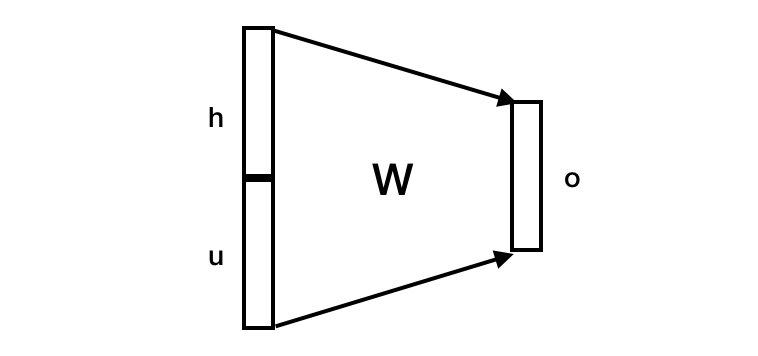
\includegraphics[width=0.4\linewidth]{连接融合.png}
  \caption{连接融合}
\end{figure}

如上图所示,连接融合是将两个向量串联,即$[u,h]$,最后在引入一个维度平衡矩阵$W$,
将其映射为原先的维度.

\begin{equation}
  o = W[u,h]
\end{equation}




\chapter{实验部分}
为了检验融合模型在文本理解中的效果,选择最为基础的文本分类任务.
在公开的文本分类数据集上进行了传统机器学习方法KNN、SVM、RNN、LSTM模型和融合模型的对照实验.
进一步对融合模型的中的超参数,Attention和融合方式进行了对照实验.

\section{实验准备}
\subsection{实验环境}
本文的实验
传统机器机器学习方法基于机器学习库sklearn实现,
深度学习相关的模型基于Google的开源深度学习库Tensorflow.
其中Tensorflow是基于图的计算框架,数据(Tensor)在节点中流动,
并在节点内部完成计算,所以可以很方便的实现模型搭建,训练,测试等任务.
本文具体的实验环境见下表:

\begin{table}[h!]
  \centering
  \begin{tabular}{cccc}
    \toprule
    \textbf{类别} & \textbf{描述} & \textbf{类别} & \textbf{描述}\\
    \midrule
    开发语言 & Python3.6  & 开发框架 & Tensorflow1.2\\
    操作系统 & Red Hat 4.8.5 & 硬盘大小 & 150 TB \\
    GPU型号 & NVIDIA TITAN X & 显存大小 & 11 GB \\
    CPU型号 & Intel E5-2683 v3(56核) & 内存大小 & 600 GB\\
    \bottomrule
  \end{tabular}
  \caption{实验环境}
\end{table}

\subsection{数据集}
新闻数据是目前互联网数据中最为庞大的一部分,所以很适合作为文本分类的实验对象.
这里选择AGNews语料公开数据集,数据可以在官网上下载.
整个数据集包括了从超过2000个数据源上获取的一共496835则新闻语料.
本文选择了语料中的4个最大类别来形成数据集.
4个类别的数据集一共有12000训练数据,7600测试数据,
在此基础上,随机从训练数据集上选择了10000条作为开发集数据
具体见下表.

\begin{table}[h!]
  \centering
  \begin{tabular}{ccccc}
    \toprule
    \textbf{类别} & \textbf{总体} & \textbf{开发集} & \textbf{测试集} & \textbf{测试集} \\
    \midrule
    World & 31900 & 27451 & 2549 & 1900 \\
    Sports & 31900 & 27503 & 2497 & 1900 \\
    Business & 31900 & 27541 & 2459 & 1900 \\
    Sci/Tech & 31900 & 27505 & 2495 & 1900 \\
    \bottomrule
  \end{tabular}
  \caption{AGNews数据集}
\end{table}

具体来说,一则新闻数据包括标签和文本.例如:
"3","Surviving Biotech's Downturns","Charly Travers offers advice on withstanding the volatility of the biotech sector."
这里的3,表示第三类也就是Business类别,对于文本内容,
由新闻的标题和新闻描述两个部分构成.数据集数据示例如下图所示:

\begin{figure}[h!]
  \centering
  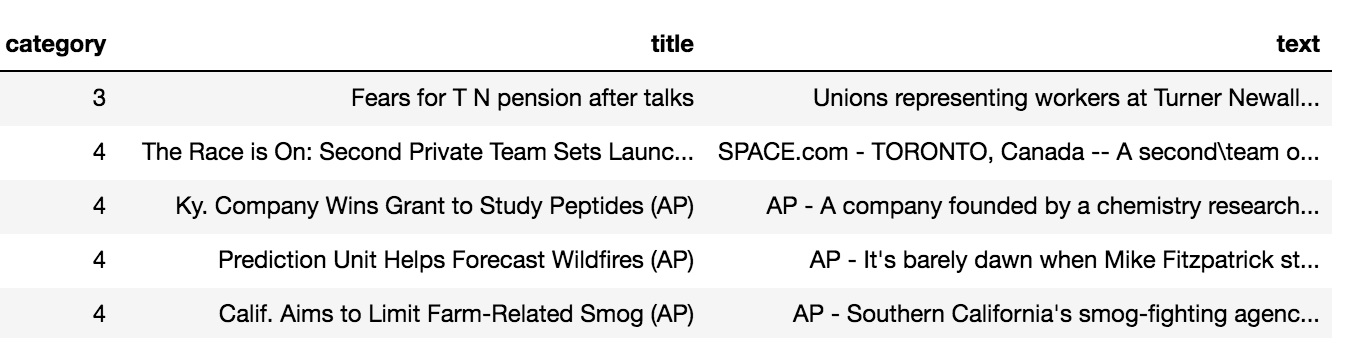
\includegraphics[width=0.8\linewidth]{数据示例.png}
  \caption{数据集数据示例}
\end{figure}


所以需要对文本内容进行一步预处理,首先需要将标题和描述构成一个长的新文本,
然后对于单词全部转成小写形式并去除标点符号.
注意,这样的操作不会改变文本本身的句法结构特征的.
这样新闻文本的长度分布如下图所示:

\begin{figure}[h!]
  \centering
  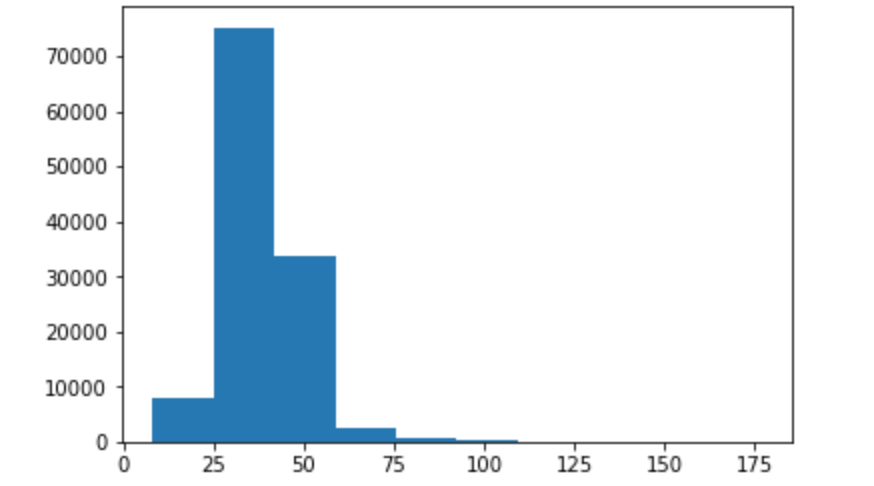
\includegraphics[width=0.6\linewidth]{长度分布.png}
  \caption{新闻长度分布}
\end{figure}

经过计算文本平均长度为37.8,绝大多数在100词以内.
所以可以设置参数最大序列长度$max\_seq\_length$,超过最大长度则截取超出部分,
不足则补充空值.
这样将清洗后的文本通过词向量矩阵映射,就可以获得文本的词向量表示,
这也是最终送入模型的文本形式.映射过程如下图所示.

\begin{figure}[h!]
  \centering
  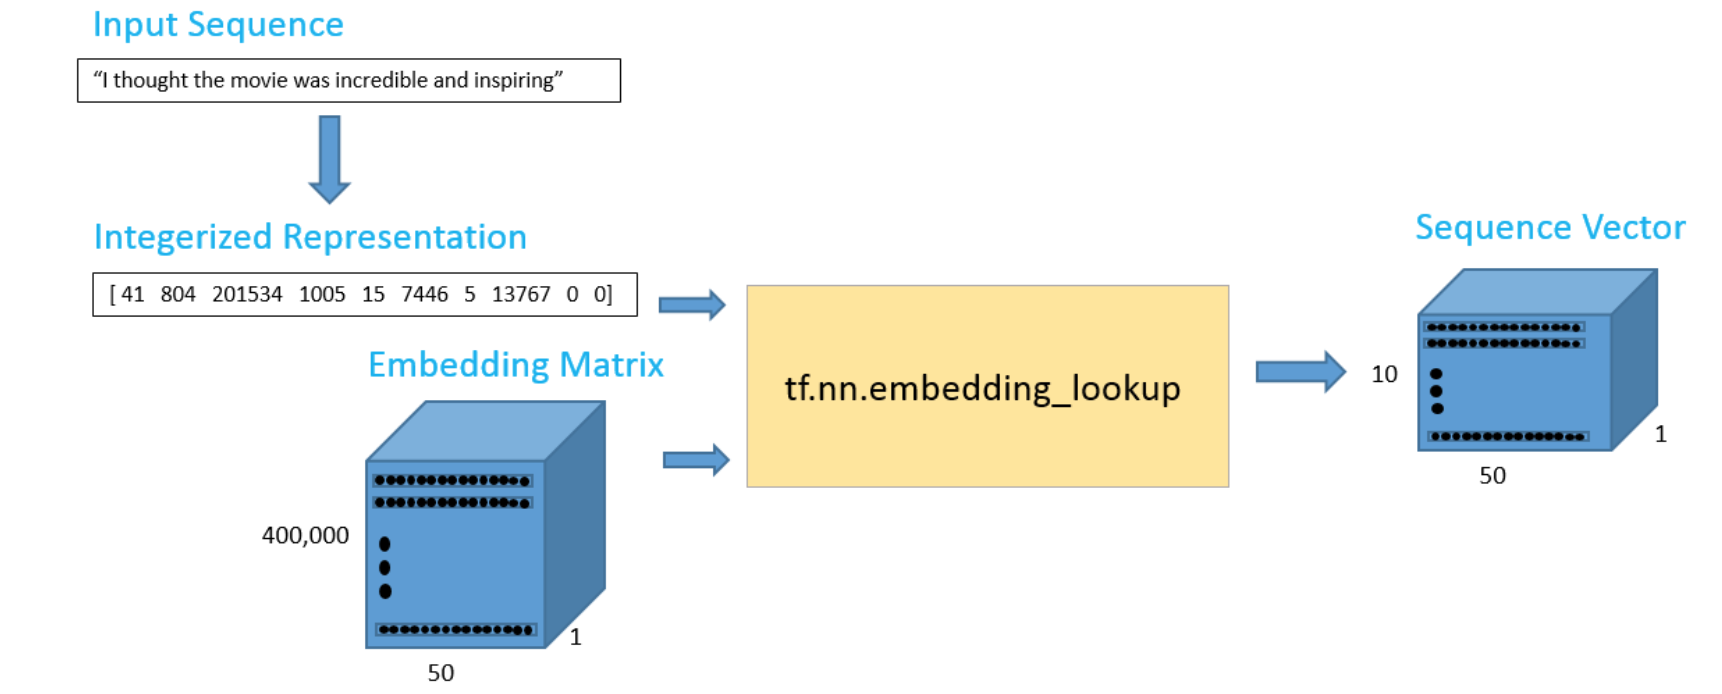
\includegraphics[width=0.95\linewidth]{词向量映射.png}
  \caption{文本向量化}
\end{figure}


\subsection{实验模型}
实验模型采用融合模型,后面接入一层全连接的神经网络,最后通过softmax计算每个类别的概率.
实验模型图示如下:
\begin{figure}[h!]
  \centering
  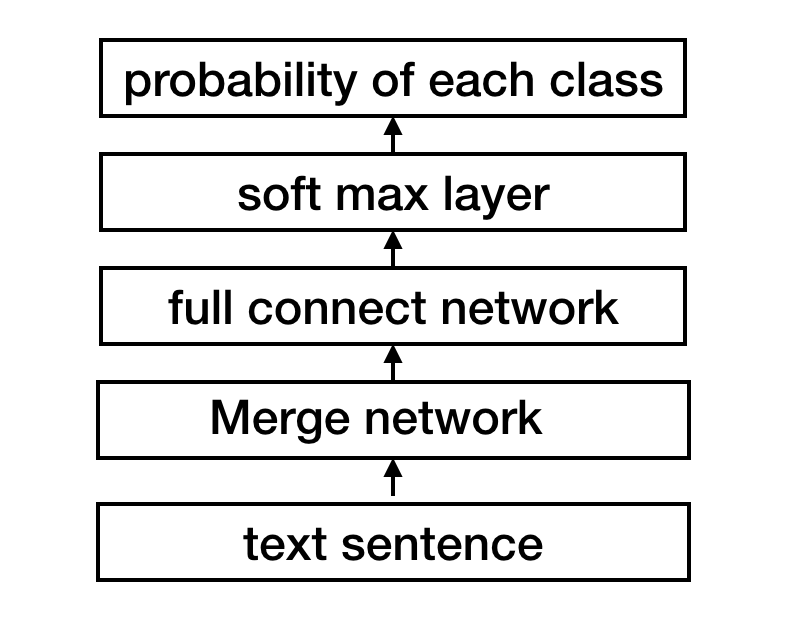
\includegraphics[width=0.4\linewidth]{分类模型.png}
  \caption{实验模型图示}
\end{figure}

模型采用Adam优化算法\cite{Kingma2014Adam}进行训练.

在实验中可以采用动态RNN的方法,
即每句话根据自己的长度在RNN中循环多少次,而不需要循环后续补充的0.
这样可以提高模型训练速度,同时可以避免填充的空值对语义的理解.

实验中的超参数配置具体如下表所示,

\begin{table}[h!]
  \centering
  \begin{tabular}{cccc}
    \toprule
    \textbf{超参数} & \textbf{取值} & \textbf{超参数} & \textbf{取值}  \\
    \midrule
    hidden\_layers & 1 & hidden\_size & 128 \\
    batch\_size &  50 & max\_iterations & 5000 \\
    word\_embedding\_dimension & 50 & max\_seq\_length & 100 \\
    full\_connect\_network\_layers & 1 & leanring\_rate & 0.001 \\
    \bottomrule
  \end{tabular}
  \caption{实验超参数表}
\end{table}

值得注意的是,对于上表中超参数的调整必然可能影响实验的结论,
比如增加词向量的维度从50维度提升到200维度,或者增加隐藏层的大小,
但是这些超参数的研究并不在实验讨论的范围中,因为实验的目的是为了对比
融合模型和RNN、LSTM模型,而因为融合模型中的核心就是两个LSTM模型,
所以这些超参数的调整会同步改变所有模型的结果.

所以后续实验中融合模型和RNN、LSTM模型的超参数均基于上表,以此来进行实验对照.
后面实验中获得的最佳结果也仅仅是基于这个超参数表获得的最好结果.

最后实验代码开源在GitHub上:https://github.com/SimpleBrightMan/GraduateProject/
如果在复现实验过程中遇到问题,或者有更好的结果,欢迎直接在网页上开issue向我反馈.

\section{实验结果和分析}
\subsection{基础实验}
基础实验采用传统的机器学习模型SVM,KNN,RNN,LSTM和本文提出的融合模型进行了对照实验.

传统机器学习模型,SVM,KNN模型词向量是直接统计整个语料库中的词频作为词向量.
其中SVM模型采用最基本的线性核,而KNN对于近邻的权重,采用权重一样的方式.
深度学习相关的模型,在训练集上训练模型,每隔5步保存模型,并计算在开发集上的正确率,
最终取开发集上正确率最高的模型,计算其在测试集上的正确率.
对于融合模型基础实验部分采用的是dot Attention和简单的加和融合方式.
最终结果如下表所示,

\begin{table}[h!]
  \centering
  \begin{tabular}{cccc}
    \toprule
    \textbf{模型} & \textbf{开发集最大准确率} & \textbf{测试集准确率} \\
    \midrule
    KNN & 88.70\% & 86.30\% \\
    SVM & 94.80\% & 87.19\% \\
    RNN & 87.59\% & 85.60\% \\
    LSTM & 91.00\% & 88.31\% \\
    融合模型 & 94.20\% & 90.50\% \\
    \bottomrule
  \end{tabular}
  \caption{基础实验结果}
\end{table}


可以看出整体上看传统机器学习模型中SVM模型能取得较好的结果,
所以事实上SVM在先前也一直用来处理文本分类任务.
在深度学习模型中传统的RNN效果最差,主要是因为新闻语料的文本是属于长文本的,
LSTM相对于RNN有较大的提升,提高了接近3\%的测试集准确率,
最后本文提出的融合模型,实验效果最好,达到了90.50\%的准确率.
进一步绘制融合模型的分类混淆矩阵,如下图所示.

\begin{figure}[h!]
  \centering
  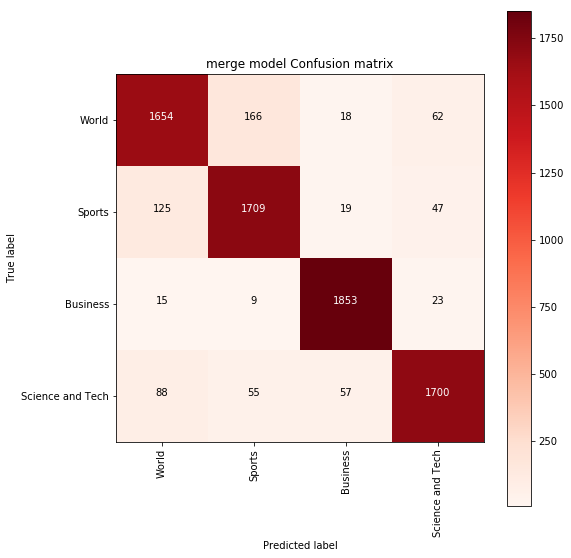
\includegraphics[width=0.45\linewidth]{混淆矩阵.png}
  \caption{融合模型分类混淆矩阵}
\end{figure}

从分类混淆矩阵可以看出实际上Word和Sports两个类别比较容易相互分类错误.

进一步分析训练数据大小对不同深度学习模型的影响,
以评价在训练数据集有限的情况下模型的效果.
选取训练数据集分别为5k、10k、15k和20k,开发集固定为2.5k,测试集为依然为1.9k.
比较测试集准确率,实验结果如下表所示:

\begin{table}[h!]
  \centering
  \begin{tabular}{ccccc}
    \toprule
    \textbf{模型} & \textbf{5K} & \textbf{10K} & \textbf{15K} & \textbf{20K}\\
    \midrule
    RNN & 80.05\% & 82.12\% & 83.96\% & 85.26\%\\
    LSTM & 82.70\% & 85.92\% & 87.03\% & 88.42\%\\
    融合模型 & 86.81\% & 87.30\% & 88.70\% & 90.40\%\\
    \bottomrule
  \end{tabular}
  \caption{不同规模训练数据模型在测试集上准确率}
\end{table}

可以看出融合模型在不同规模的数据集上均获得了最佳的结果.
并且值得注意的是,在小规模数据集上,由于融合模型因为了语言学的先验知识,
所以相较于LSTM模型,提升了4\%,具有明显的优势.

再进一步分析RNN,LSTM和融合模型的训练过程.
这三个模型在迭代过程中迭代次数和开发集准确率、训练集上的loss的变化曲线如下

\begin{figure}[h!]
  \centering
  \begin{subfigure}[b]{0.8\linewidth}
    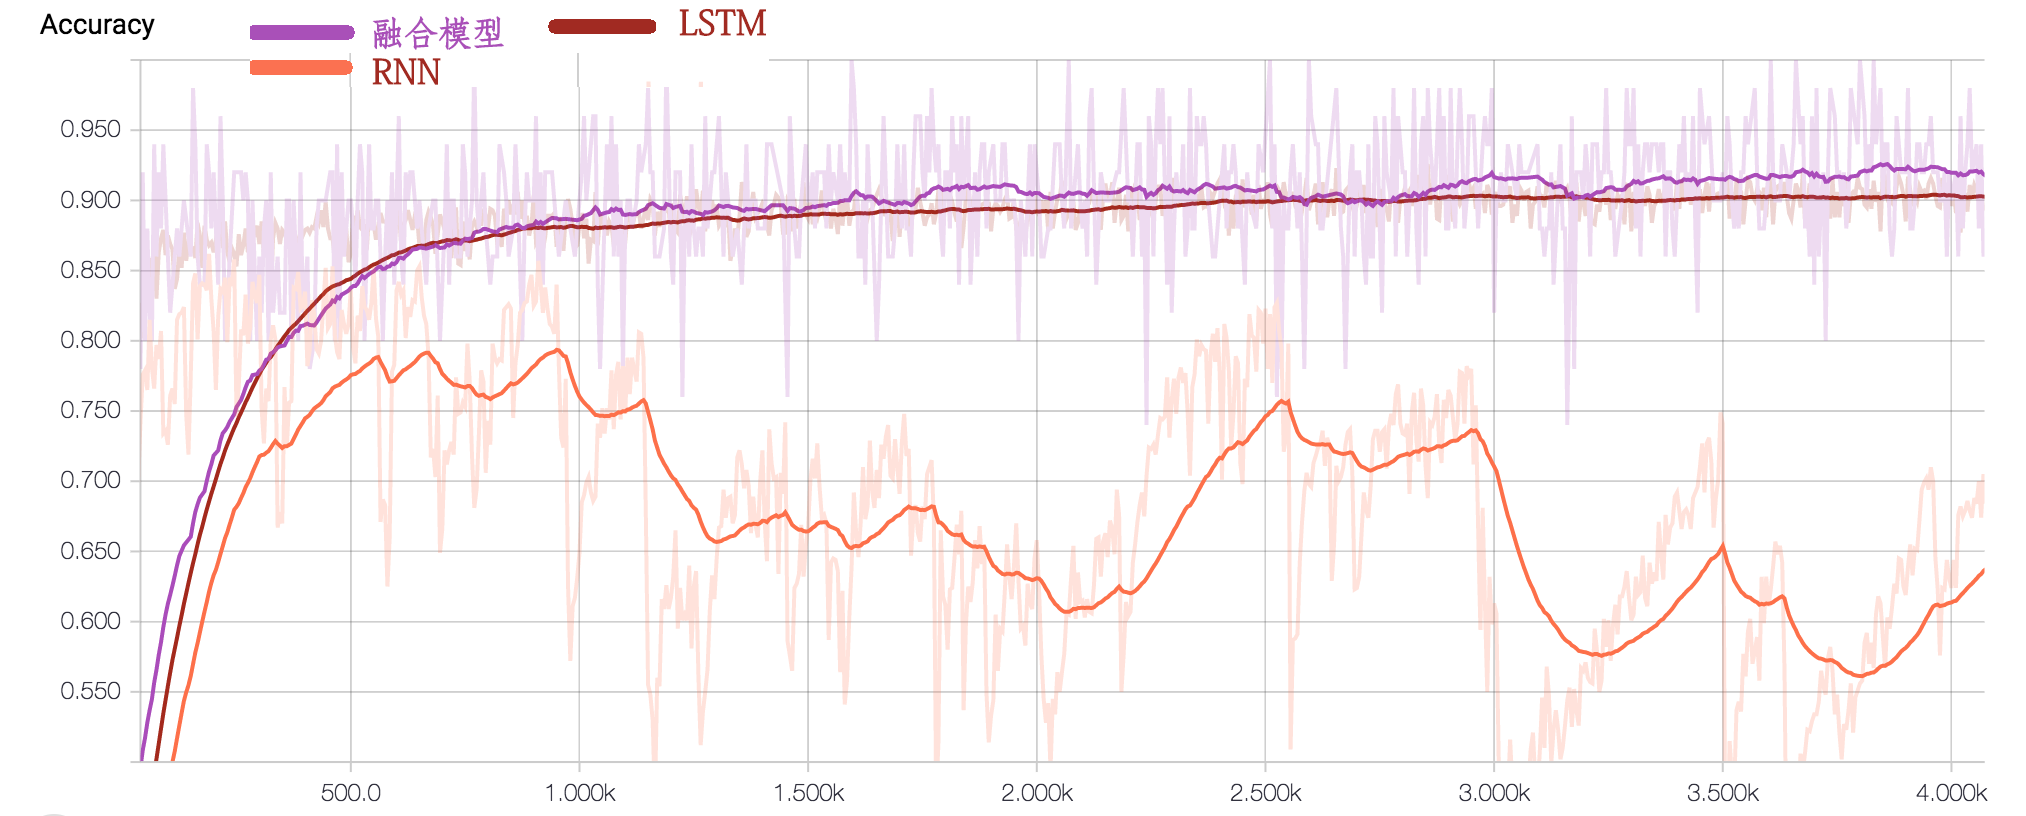
\includegraphics[width=\linewidth]{accuracy-1.png}
    \caption{开发集准确率变化}
  \end{subfigure}
  \begin{subfigure}[b]{0.8\linewidth}
    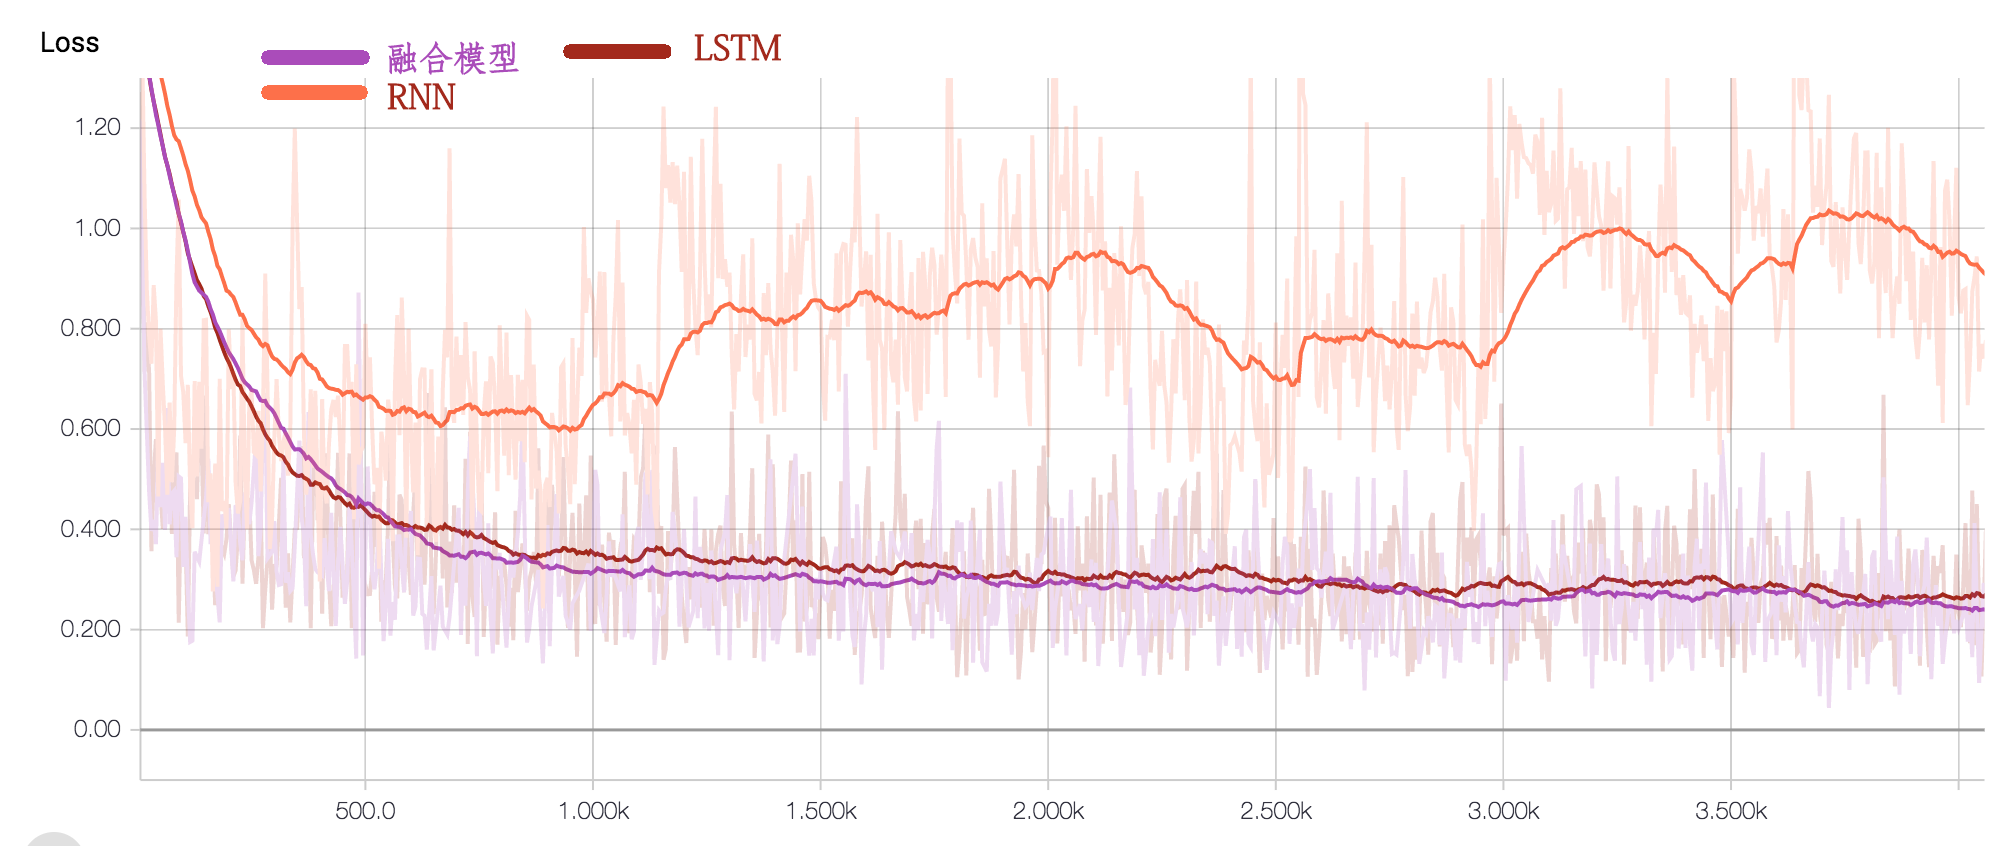
\includegraphics[width=\linewidth]{loss-1.png}
    \caption{训练集loss变化}
  \end{subfigure}
  \caption{迭代次数和准确率、loss的变化曲线}
\end{figure}

从图中可以看出RNN模型和另外两个模型差距明显,
融合模型和LSTM模型相比,从图中来看,
迭代的整个过程中准确率基本一直比LSTM模型更高,loss则更低.

局部观察迭代初期较少次的训练和迭代后期趋于稳定以后开发集准确率的对比,
如下图所示:

\begin{figure}[h!]
  \centering
  \begin{subfigure}[b]{0.8\linewidth}
    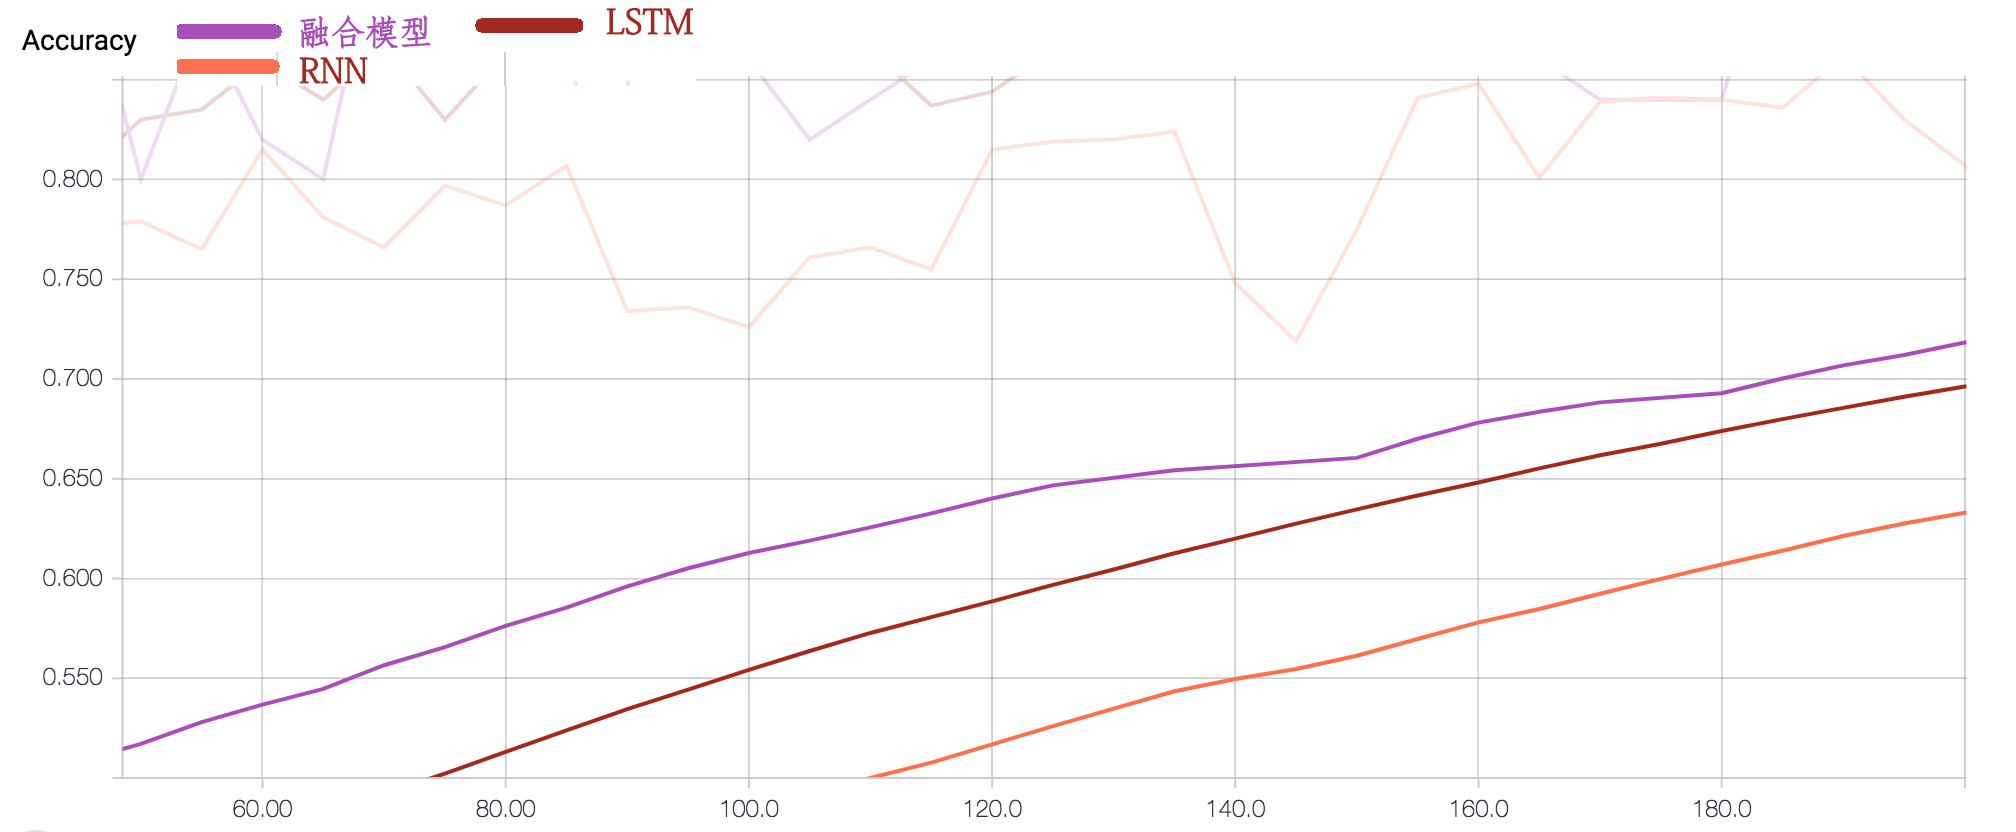
\includegraphics[width=\linewidth]{基本-准确率初期.png}
    \caption{迭代前期准确率对比}
  \end{subfigure}
  \begin{subfigure}[b]{0.8\linewidth}
    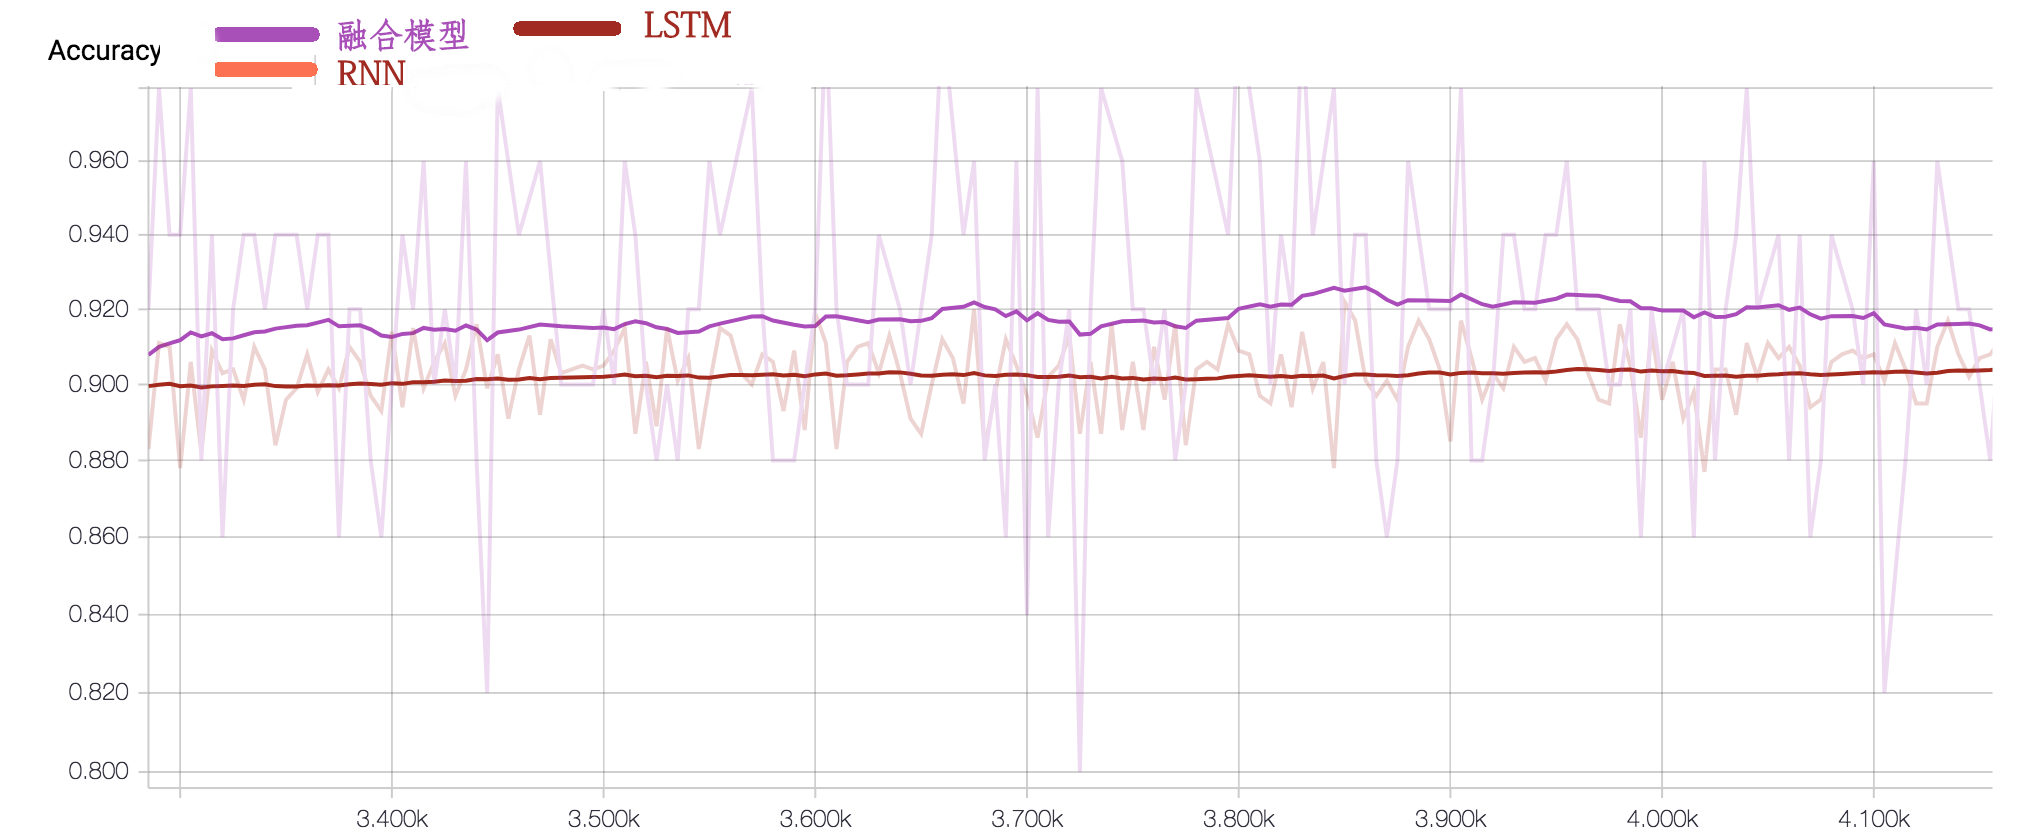
\includegraphics[width=\linewidth]{基本-准确率后期.png}
    \caption{迭代后期准确率对比}
  \end{subfigure}
  \caption{迭代前期与后期融合模型和LSTM模型开发集准确率对比}
\end{figure}

从上图可以看出,在迭代初期,120次迭代的情况下,融合模型准确率在65\%附近,
而LSTM在60\%,高出5个百分点;在迭代后期,3800次迭代以后,模型区域稳定,
可以看到融合模型的准确率一直稳定在92\%在附近,而LSTM模型在稳定在90\%,
高出2个百分点.所以融合模型在迭代前期和后期均优于LSTM模型,并且在前期迭代效率更高.

最后对比模型的训练速度,在训练的过程中,可以预先将每个句子解析成依存句法结构,
并建立根据文本获得子结构的映射字典,这样获取句法解析的时间复杂度就是O(1).
所以在训练过程中不需要在线解析,训练速度可以大幅度提高融合模型训练的时间.
但是在测试环节,为了模拟真是环境,是不知道测试数据的,所以必须在线解析句法结构.

实验环境见表4-1,模型超参数配置见表4-3,
统计训练迭代1000次和测试1000个数据的耗时,
具体每个模型的速度对比如下表所示.可以看出融合模型的训练时间和测试时间均是最长的,
训练时间上融合模型是LSTM耗时的3倍,是RNN模型的近8倍;
而测试时间融合模型是LSTM和RNN模型的4倍多.
但是由于在GPU上训练模型,数据量不是巨大,
所以在实验过程中定性的看差距不是巨大,但是确实融合模型的复杂度提升以后,
在线处理的实时性被一定程度削弱.

\begin{table}[h!]
  \centering
  \begin{tabular}{ccc}
    \toprule
    \textbf{模型} & \textbf{训练时间(1K迭代)} & \textbf{测试时间(1K数据)}\\
    \midrule
    RNN &  12.71min & 18.49s \\ 
    LSTM & 30.92min & 20.78s \\ 
    融合模型 & 93.53min & 82.80s \\ 
    \bottomrule
  \end{tabular}
  \caption{模型速度比较}
\end{table}


\subsection{Attention对比实验}
针对子结构的Attention进行了进一步对照实验,分别选择了
无Attention,就是直接平均、dot Attention、bi-liner Attention和
concatenation-based Attention.实验结果见下表.

\begin{table}[h!]
  \centering
  \begin{tabular}{cccc}
    \toprule
    \textbf{Attention} & \textbf{开发集最大准确率} & \textbf{测试集准确率} \\
    \midrule
    无Attention & 92.90\% & 89.25\% \\
    dot Attention & 94.20\% & 90.65\% \\ 
    bi-liner Attention & 93.50\% & 90.50\% \\
    concatenation-based Attention & 93.50\% & 90.83\% \\
    \bottomrule
  \end{tabular}
  \caption{Attention实验结果}
\end{table}

可以看出有无Attention存在明显差距,无Attention在测试集上准确率低于90\%,
有Attention均高于90\%.在最终结果上concatenation-based Attention获得最佳的结果,
准确率测试集准确率达到了90.83\%.
可以进一步可视化出Attention机制,以句子”NKorea warns Japan against economic sanctions“,为例,
其子结构和Attention值如下表:

\begin{table}[h!]
  \centering
  \begin{tabular}{lc}
    \toprule
    \textbf{子结构} & \textbf{concatenation-based Attention} \\
    \midrule
    warns NKorea & 0.44 \\ 
    warns Japan & 0.41 \\
    warns sanctions against & 0.12 \\
    warns sanctions economic & 0.03 \\
    \bottomrule
  \end{tabular}
  \caption{子结构与其Attention值}
\end{table}

从而可以得倒整个句子的Attention热力图分布,如下图所示.

\begin{figure}[h!]
  \centering
  \includegraphics[width=0.6\linewidth]{Attention图.png}
  \caption{Attention可视化}
\end{figure}

可以看出在句子中核心重要的词,除去动词warns,就是两个国家名
NKorea和Japan,所以其分类也是World.
通过上面的可视化,使得模型有了很好的解释性.

\subsection{融合方式对比实验}
针对融合方式进行了进一步的实验,主要是相加融合和连接融合,这里选取Attention最好的
结果concatenation-based Attention,实验结果如下:

\begin{table}[h!]
  \centering
  \begin{tabular}{cccc}
    \toprule
    \textbf{融合方式} & \textbf{开发集最大准确率} & \textbf{测试集准确率} \\
    \midrule
    相加融合 & 93.50\% & 90.83\% \\
    连接融合 & 93.90\% & 90.66\% \\
    \bottomrule
  \end{tabular}
  \caption{融合方式实验结果}
\end{table}

可以看出相加融合和连接融合差不并不是很大,
但是相加融合的方式在测试集上取的效果更佳.
对于相加模型,进一步进行有权重的相加,也就是$o = \alpha u + (1-\alpha)h$,权重$\alpha$,取值为$[0.1,0.9]$,步长为$0.1$.
实验结果如下:
\begin{table}[h!]
  \centering
  \begin{tabular}{ccccccc}
    \toprule
    \textbf{$\alpha$取值} & \textbf{开发集最大准确率} & \textbf{测试集准确率} & \textbf{$\alpha$取值} & \textbf{开发集最大准确率} & \textbf{测试集准确率} \\
    \midrule
    0.1 & 93.30\% & 90.20\% & 0.2 & 93.90\% & 90.21\%\\
    0.3 & 94.10\% & 90.31\% & 0.4 & 94.30\% & 90.43\%\\
    0.5 & 94.10\% & 90.27\% & 0.6 & 93.90\% & 90.18\%\\
    0.7 & 94.40\% & 90.86\% & 0.8 & 94.30\% & 90.67\% \\
    0.9 & 94.80\% & 90.47\% &&&\\
    \bottomrule
  \end{tabular}
  \caption{不同权重$\alpha$实验结果}
\end{table}

绘制权重$\alpha$与测试集准确率的变化曲线.

\begin{figure}[h!]
  \centering
  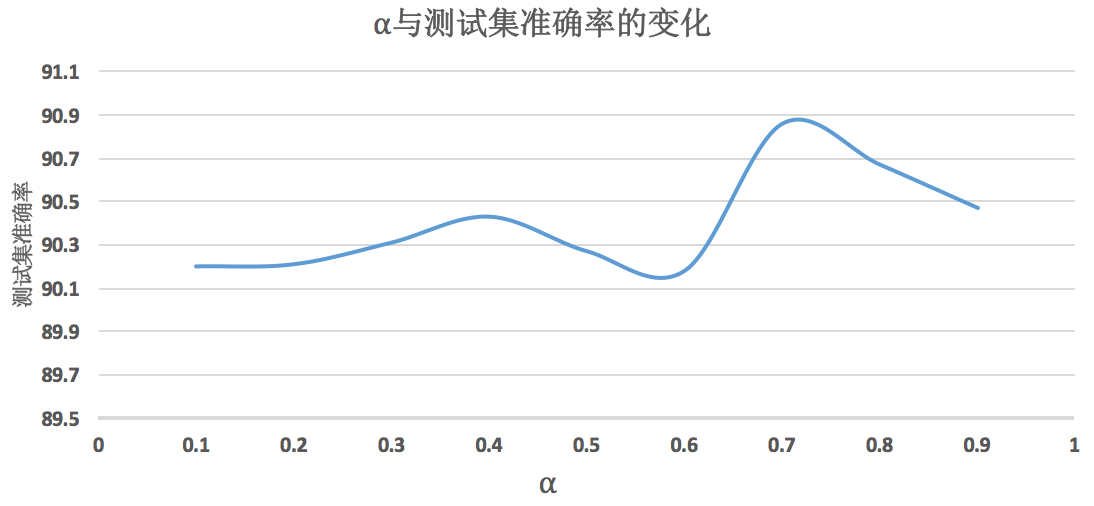
\includegraphics[width=0.6\linewidth]{权重变化.png}
  \caption{权重$\alpha$与测试集准确率变化曲线}
\end{figure}

可以看出整体上测试集准确率随着$\alpha$先增后降,并在
$\alpha = 0.7$的时候获取最大值,90.86\%,
这也是融合模型获得的最好结果.
这个结果相比LSTM的结果提升了2.5个百分点.

\chapter{结论与展望}
\section{结论}
文本内容理解作为自然语言处理领域的一项核心技术,其研究在理论和实际应用
上都有重要的意义.
文本内容理解的主要任务是对序列建模,构建模型可以“学习”文本内在的表示特征.
当前基于RNN、LSTM等深度学习模型已经成为了主流方式,但是这种方式忽略了文本自身的语言学知识,
需要非常大的数据集而且缺乏可解释性和鲁棒性.

本文的主要工作是提出了融合依存句法结构的深度神经网络模型,并将模型运用的文本分类的具体应用上,
比传统的神经网络模型取得了更好的效果.

总的来说,通过文本分类的实验,可以看出融合模型具有下面几个优势:

(1) 因为融合模型学习了语言学知识,
所以在小规模数据集上融合模型的实验效果相对于RNN、LSTM模型有明显的提升,测试集上准确率提升4\%,
在大数据集上融合模型也具有有优势,测试集准确率最高提升2.5\%.

(2)通过引入Attention机制使得模型可以可视化出在
分类任务上文本中每一个子结构的重要程度,也就进一步可以可视化出
文本中的每一个单词的重要程度.通过可视化文本Attention的热力图,
使得模型具备一定的解释性.

(3)融合模型的迭代效率更高,在迭代初期,100次迭代左右,就能获得很好的
实验效果,比RNN、LSTM模型能高出5\%的准确率.

(4)该模型引入依存句法作为语言学知识,
将融合模型的输出结果融合向量表示,可以送入后续任何形式的网络中,
来完成众多不同的文本理解任务.
并且该模型可以无缝替换原先的RNN、LSTM模型,因为融合模型和其输入输出形式完全相同,
所以可以很方便的升级原先的模型,将语言学知识引入原先的模型中.

本文还对模型的Attention方式和融合方式进行了深入的研究,实验表明
采用concatenation-based Attention和加权融合能产生最好的实验结果,
相对LSTM模型提升了2.5\%的准确率.

\section{不足与展望}
因为文本内容理解本身就是一件复杂的研究领域,所以由于条件和时间等方面的原因,
本文的方法还存在需要改进和完善的地方,主要如下:

(1)该模型目前仅仅在在文本分类的任务上进行了实验,还未在更多的文本内容理解任务上实验,
所以可能在某些其他任务上实验效果会不如人意.
尤其对于中文依存句法的解析效果目前还不如英语,所以本模型在处理中文语境下可能会较差,
当然这需要进一步实验来改进调整模型.

(2)该模型由两个独立的LSTM模型和依存句法解析工具构成,所以模型复杂度较高,
在在线处理文本上实时性相对于传统RNN、LSTM模型较差.
主要性能瓶颈在句法解析上,所以未来可能考虑将句法解析融入网络中,
或者引入性能更高的句法解析工具.


% 参考文献.应放在\backmatter之前.
% 推荐使用BibTeX,若不使用BibTeX时注释掉下面一句.
\nocite{*}
\bibliography{bachelor}
% 不使用 BibTeX
%\begin{thebibliography}{2}
%
%\bibitem{deng:01a}
%{邓建松,彭冉冉,陈长松}.
%\newblock {\em \LaTeXe{}科技排版指南}.
%\newblock 科学出版社,书号:7-03-009239-2/TP.1516, 北京, 2001.
%
%\bibitem{wang:00a}
%王磊.
%\newblock {\em \LaTeXe{}插图指南}.
%\newblock 2000.
%\end{thebibliography}

%%%%%%%%%%%%%%%%%%%%%%%%%%%%%%%%%%%%%%%%%%%%%%%%%%%%%%%%%%%%%%%%%%%%%%%%%%%%%%%
% 致谢,应放在《结论》之后
\begin{acknowledgement}
  
\end{acknowledgement}

\backmatter




%%%%%%%%%%%%%%%%%%%%%%%%%%%%%%%%%%%%%%%%%%%%%%%%%%%%%%%%%%%%%%%%%%%%%%%%%%%%%%%
\end{document}
